\documentclass{article}
\usepackage[dblblindworkshop,final,nonatbib]{neurips_2026}
\workshoptitle{Agentic AI for Biological \mbox{Discovery} (AgenticLS)}
\usepackage[numbers,sort&compress]{natbib}
\usepackage{cmap}
\usepackage[T1]{fontenc}
\usepackage[utf8]{inputenc}
\usepackage{booktabs,amsmath,amssymb,amsthm,graphicx,microtype,tabularx}
% placeins' \FloatBarrier keeps each appendix's tables inside it
\usepackage{placeins}
\newtheorem{lemma}{Lemma}
\newtheorem{remark}{Remark}
\newtheorem{observation}{Observation}
\usepackage[hidelinks]{hyperref}
\hypersetup{pdftitle={Forced Choice Is Not a Tolerance: What Multiple-Choice Grading Accepts on BixBench's Numeric
  Questions}, pdfauthor={Vijayavallabh Jayamanikandan}}
\title{Forced Choice Is Not a Tolerance\protect\\What Multiple-Choice Grading Accepts on BixBench's Numeric Questions}
\author{%
  Vijayavallabh Jayamanikandan\\
  Indian Institute of Technology Madras\\
  \texttt{be23b041@smail.iitm.ac.in}
}

\exhyphenpenalty=10000
\begin{document}
\maketitle

\begin{abstract}
BixBench, a benchmark of biological data analysis for agents, grades an agent's free-text answer in two ways:
open-ended, and through multiple choice, where a second model reads the agent's notebook and answer and selects one of
four options, either forced to choose or allowed to refuse. A 2026 system still reports the forced-choice score. On
the benchmark's numeric questions, we compare the multiple-choice grades with a tolerance, which accepts a submitted
number within $5\%$ of the correct value (the \emph{key}), on the runs BixBench published and on runs of open-weight
and current agents. Forced to choose, BixBench's grader accepts $17$ to $25\%$ of the wrong answers, about as many as a
random choice among four would, but it favours those whose nearest option is the key: on the published runs of gpt-4o
and Claude 3.5 Sonnet, it accepts these $3.5$ and $6.0$ times as often as wrong answers nearest a wrong option. On
three current agents' runs, forced choice still scores $10$ to $12$ percentage points above the tolerance. The standard correction
for guessing matches the tolerance on the published runs only because opposite errors cancel. The options also reveal
where the key lies: in the second release, v1.5, the key is the second-smallest of the four values on $51\%$ of numeric
questions, and a rule that ignores the question learns this rank from the benchmark's other datasets. Drawing the key's
rank at random would hide it, but it conflicts with rejecting wrong answers: some keys then become the smallest or
largest option, and every wrong answer of the same sign beyond such a key is nearest to it. Graders accept such answers
to the extent that they select the option nearest the answer. Numeric answers should be graded by tolerance.
\end{abstract}

\section{Introduction}
\label{sec:intro}

BixBench \citep{bixbench} asks an agent to analyse a biological dataset in a notebook and submit a free-text answer,
which it grades open-ended and through multiple choice. In multiple choice, a second model, the \emph{multiple-choice
grader}, receives the notebook, the question with four options and the answer, and selects the best option, either
\emph{forced} to choose or allowed to \emph{refuse} by selecting ``Insufficient information to answer the question''. One option, the
\emph{key}, is correct; the other three are \emph{distractors}. BixBench's authors call the options ``a useful proxy''
whose scores are ``marginally better than random'', yet the forced-choice score remains in use: a 2026 system
\citep{bioagents} reports $64.4\%$ forced-choice and $48.8\%$ open-ended accuracy on v1.5, BixBench's second release
(v1.0 was the first). Its forced-choice grader sees the answer and the options but not the notebook, yet the score is set
beside published forced-choice scores graded with the notebook. No one has measured how much of such a score comes
from wrong answers that the grader accepts.
\begin{figure}[t]
\centering
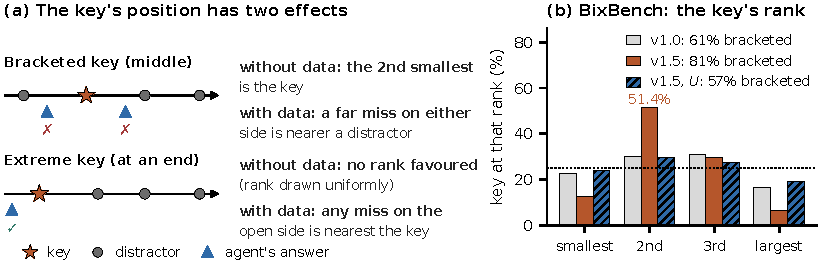
\includegraphics[width=\linewidth]{figures/overview.pdf}
\caption{\textbf{Options that reject misses on both sides reveal the key's rank.}
\textbf{(a)} With a distractor on each side (a \emph{bracketed} key), the key (star) has a middle rank, which a
rule that ignores the question can learn; an answer (triangle) that misses by more than half the log-scale gap to the
next option on either side is nearer a distractor. A key that is the smallest or largest option (an \emph{extreme} key)
need not reveal its rank, but every miss beyond it on its side with no distractor (the \emph{open side}) is nearest
it.
\textbf{(b)} BixBench v1.5's $105$ numeric items: the key is the second-smallest of four values on $51.4\%$ of them;
$81\%$ are bracketed, against $61\%$ of v1.0's $159$ and $57\%$ under $U$, the rewrite that draws the key's rank at
random (\S\ref{sec:theory}); dotted line: $25\%$, a uniform rank.}
\label{fig:overview}
\end{figure}

We measure it on the questions whose options are numbers (the \emph{numeric items}: $159$ in v1.0 and $105$ in
v1.5), where correctness needs no grader: a \emph{tolerance} accepts the submitted number, the last number in the answer, if
it lies within $5\%$ of the key \citep{scibench}, and any other answer, including one with no number, is a \emph{miss}.
Because the agent never sees the options, we can regrade its answers through other option sets after the run
(Figure~\ref{fig:design}). BixBench groups its questions into \emph{capsules}, each a dataset with its questions. The key's \emph{rank} is its place among the sorted option values. We find that:
\begin{itemize}\setlength{\itemsep}{1pt}\setlength{\topsep}{2pt}\setlength{\parsep}{0pt}
\item forced choice accepts about as many misses as a random choice would, but favours those whose nearest option is
the key (\S\ref{sec:withdata}, Table~\ref{tab:released});
\item the standard correction for guessing agrees with the tolerance only because opposite errors cancel
(\S\ref{sec:guessing});
\item v1.5's options reveal the key's rank (\S\ref{sec:leak}, Figure~\ref{fig:overview}b);
\item drawing the rank at random would hide it, but for a grader that \emph{follows the nearest option}, selecting
the option nearest the submitted number, this conflicts with rejecting misses (Observation~\ref{obs:bracket},
Figure~\ref{fig:overview}a);
\item real graders bear this cost to the extent that they follow the nearest option (\S\ref{sec:cost}), and no design of
the option values escapes it (\S\ref{sec:design}).
\end{itemize}

\section{Related work}
\label{sec:related}

\emph{Grading free-text answers.} Comparing an answer with the correct one agrees with human grading where
multiple choice does not \citep{answermatching,openstyle}; for a number the comparison is a tolerance
\citep{scibench}. Automatic answer checkers
miss answers written in another form or accept wrong ones \citep{xverify,compassverifier,verifierpitfalls}, models used
as judges are biased and lenient \citep{llmjudge,fairevaluators,judgingjudges}, and the standard correction for
guessing, formula scoring \citep{lordformula,frary}, assumes that guesses fall on the options at random. \emph{Choices
without the question.} BixBench's no-data baseline, the score of a model that answers without the data, is a
multiple-choice form of the hypothesis-only baseline, which asks what a model can answer from part of its input
\citep{hypothesisonly,artifacts}, here the options \citep{choicesonly,shortcut,rightwrong,niven}. ``Choose the middle
value'' is a cue test-takers learn \citep{testwiseness}. Shuffling the order in which options are shown removes cues in
an option's position \citep{attalibarhillel,selectionbias,positionsensitivity} but not this one, which lies in the
values, not in their order.
Work on distractors asks how well they attract test-takers who do not know the answer
\citep{haladynataxonomy,haladynarodriguez,distractorgeneration,distractorfunction,howmanyoptions,threeoptions}, and
contamination tests ask whether a model has seen the test
\citep{memorisationexploitation,contaminationsurvey,taskcontamination,minkprob,memorisation,timetravel,tsguessing,exchangeablecontamination};
neither asks what the options reveal without the question. \emph{Agent benchmarks} have been criticised for lacking
held-out test sets and for grading that misestimates performance \citep{agentsmatter,abc}. A concurrent audit of
BixBench \citep{bixbenchaudit} re-derives the answer keys of three capsules ($14$ questions) from the raw data and
grades $140$ replicated agent runs on them, taking the options as given. BixBench-Verified-50 has domain experts re-check
fifty of its questions, keeps their distractors and grades the free-text answer, $13$ of the $50$ by a numeric range
\citep{verified50}; frontier agents with added skills now answer $84$ to $98\%$ of them \citep{zhang2026}. Other
benchmarks for scientific data analysis grade without options \citep{corebench,discoverybench,scienceagentbench} or
show the options to the model that answers \citep{labbench}. None measures what a forced-choice grade of a free-text
answer is made of.

\section{Methods}
\label{sec:methods}

\begin{figure}[t]
\centering
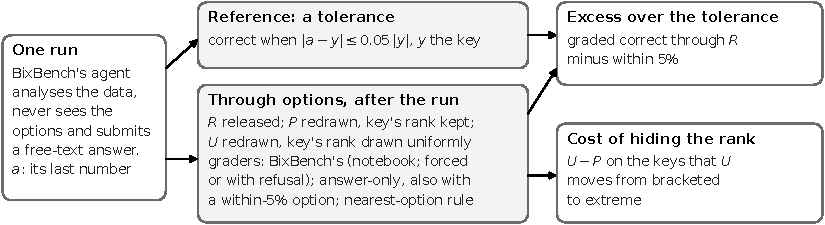
\includegraphics[width=\linewidth]{figures/design.pdf}
\caption{\textbf{What is compared.} Each answer given with the data (Table~\ref{tab:runs}) is graded by the tolerance
on its last number and, after the run, by model graders and the nearest-option rule through three option sets with the
same key ($R$, $P$ and $U$; \S\ref{sec:theory}). Table~\ref{tab:released} gives how far each grading exceeds the
tolerance; Table~\ref{tab:cost} and Figure~\ref{fig:cost} give what hiding the key's rank costs.}
\label{fig:design}
\end{figure}

\subsection{Runs and gradings}
\label{sec:runs}

Table~\ref{tab:runs} lists the runs we grade (Appendix~\ref{app:withdata}): the v1.0 runs of gpt-4o and Claude 3.5
Sonnet that BixBench released (the \emph{published runs}; where two numbers are given for them, gpt-4o's comes first),
our v1.5 runs of open-weight models, and runs of three \emph{current agents}: gpt-5.1, gpt-6-luna and DeepSeek-V4-Pro.
A \emph{configuration} is one agent model run one way, writing its tool calls as plain text or through BixBench's own
ReAct agent; a \emph{run set} is one configuration's runs from one seed (the published runs form four run sets: each
model with and without images). Besides BixBench's grader, which reads the notebook, we use \emph{answer-only} graders,
which see the question, the options and the answer but not the notebook. They approximate, but do not reproduce, the
2026 system's grader. We also offer them a \emph{within-$5\%$ option}, a fifth option stating that none of the others is
within $5\%$ of the answer (prompts in Figure~\ref{fig:gradingprompts}, terms in Table~\ref{tab:glossary}).

\begin{table}[t]
\centering\footnotesize\setlength{\tabcolsep}{3pt}
\caption{\textbf{The runs we grade}: runs with the data, on the numeric questions. \emph{In text}: the model writes
each tool call as plain text, which our code reads; \emph{ReAct}: BixBench's own agent, which alternates a reasoning
step with a tool call passed through the model server's tool-calling interface. \emph{Multiple-choice grader}: the
grader of Table~\ref{tab:released}, given BixBench's prompt and the notebook (Qwen3-30B-A3B's runs are graded by
gemma-3-27b, as its own replies were cut off before their answer). Every set is also graded through the option sets $R$, $P$ and $U$
(\S\ref{sec:theory}) by the nearest-option rule and the graders of Table~\ref{tab:cost}. $^{\dagger}$The runs of the
pre-specified test (\S\ref{sec:stats}).}
\label{tab:runs}
\begin{tabularx}{\linewidth}{@{}lr>{\raggedright\arraybackslash}Xrl@{}}
\toprule
runs & items & agents & runs & multiple-choice grader\\
\midrule
v1.0, published$^{\dagger}$ & $159$ & gpt-4o and Claude 3.5 Sonnet, each with and without its plots shown as
images, released with the benchmark & $5{,}161$ & the agent's model\\
v1.5, seven configurations & $105$ & in text: Qwen2.5-72B, Llama-3.3-70B, gemma-3-27b; ReAct: Qwen2.5-72B,
Llama-3.3-70B, GLM-4.5-Air, Qwen3-30B-A3B & $735$ & own model; gemma-3-27b\\
v1.5, new seeds$^{\dagger}$ & $105$ & two more seeds of each in-text configuration & $630$ & gemma-3-27b\\
v1.5, Qwen3-235B-A22B$^{\dagger}$ & $105$ & two runs per question, in text & $210$ & gemma-3-27b\\
v1.5, current agents & $105$ & ReAct: gpt-5.1 (two runs per question), gpt-6-luna, DeepSeek-V4-Pro & $420$ & gpt-4o
(2024-11-20)\\
\bottomrule
\end{tabularx}
\end{table}

\subsection{Why a 5\% tolerance}
\label{sec:reference}

The $5\%$ width, which SciBench also uses, agrees with BixBench's own judgment. The $60$ v1.5 keys its authors wrote
as ranges have a median half-width of $6.1\%$, and on $5{,}161$ published answers of gpt-4o and Claude 3.5 Sonnet,
BixBench v1.0's open-ended grader and a $5\%$ tolerance disagree on $120$ ($2.3\%$; chance-corrected agreement
$\kappa=0.90$, the highest of the rules we tried, Table~\ref{tab:tolerance}).

\subsection{Option sets and what they reveal}
\label{sec:theory}

Let $p_j$ be the share of items whose key has rank $j$ among the $k$ option values. A \emph{rank rule} always selects
rank $j$, ignoring the question, and so scores $p_j$. A key is \emph{bracketed} if distractors lie on both sides of
it and \emph{extreme} otherwise. The \emph{nearest-option rule} (\emph{the rule}) uses no language model: for a
number $a$ it selects the option $v$ that minimises $d(a,v)=|a-v|/(|a|+|v|)$, which for values of the same sign is the
option nearest $a$ on a log scale. In the pre-specified test (\S\ref{sec:stats}) it reads a number only when the whole
answer is a single number (Table~\ref{tab:extraction}). To separate the key's rank from the distractors' values, we compare three option sets with
the same key: $R$, the released options, and two rewrites by one generator that sees neither the question nor the runs
(Appendix~\ref{app:options}). $P$ redraws every distractor and \emph{preserves} the key's rank; $U$ redraws them and
draws the key's rank at random, each rank equally likely (\emph{uniformly}). $U$ moves $37$ of v1.5's
$105$ numeric keys from bracketed to extreme (the \emph{moved keys}) and $12$ from extreme to bracketed (the
\emph{inward keys}), and leaves $56$ bracketed or extreme as they were (the \emph{unchanged keys}, though it may change
their rank); $P$ moves none. $U-P$, the extra share of answers a grading accepts through $U$, in percentage points
(\emph{points}), is the \emph{cost} of hiding the rank. On the moved keys it isolates the rank's effect. Over all items
it is what a benchmark would see if it drew the rank uniformly, since $U$ also moves keys inward, where the rule and
most gradings accept fewer answers.

\begin{observation}[the nearest-option rule]
\label{obs:bracket}
Let a key $y\neq0$ have its nearest options of the same sign at magnitudes $|y|/\rho_-$ and $|y|\rho_+$
($\rho_\pm>1$). The rule accepts exactly the misses of $y$'s sign whose magnitude lies between $|y|/\sqrt{\rho_-}$ and
$|y|\sqrt{\rho_+}$, and, if $y$ has no such option on one side (an extreme key), also every miss of its sign beyond it
on that side, however large. Among $k$ options, a key rank drawn uniformly leaves $2/k$ of the keys extreme in
expectation, and a rank kept off the extremes lets a rank rule gain at least $1/(k-2)-1/k=2/(k(k-2))$ over chance.
\end{observation}

The observation (proof in Appendix~\ref{app:theory}) constrains only a grader that follows the nearest option. A
tolerance of width $t$ rejects any answer more than $t$ from the key, whatever the options, and so can a grader offered
an option saying that no value is within $t$ of the answer. A grader's \emph{proximity weight}
$\lambda=(1-\delta)(qk-1)/(k-1)$ measures how far it follows the nearest option, from the share $q$ of its selections
on misses that are the option nearest the miss and the share $\delta$ of misses on which it selects no option (its reply
names no option's letter). It is $1$ for a grader that always selects the nearest option, $0$ for one that selects it no
more often than any other, and lower the more often it selects none. A grader whose $q$ and $\delta$ do not depend on the options bears the rule's cost in proportion to
$\lambda$ (Remark~\ref{rem:lambda}).

\subsection{Statistics and the pre-specified test}
\label{sec:stats}

Every interval in the main text resamples whole capsules. With few capsules of unequal size, a nominal $95\%$
interval covers the true value less often than $95\%$ of the time, so each interval is read at the level that does cover
it $95\%$ of the time on data built like its own; where no level does, we give none (Appendix~\ref{app:stats}). We also
test each difference between two gradings of the same answers by flipping the sign of each capsule's difference at
random (the \emph{sign-flip test}), and we correct the paper's ten headline findings jointly for multiple comparisons
(Table~\ref{tab:claims}). Before analysing runs that no earlier analysis had used (the published runs, and new
v1.5 runs made afterwards), we fixed six hypotheses about the nearest-option rule, each with a pass criterion, in a dated plan (Appendix~\ref{app:replication}, Table~\ref{tab:predictions}). Under
the rule, $U$ should accept more than $R$ on the moved keys (H1) but not on the unchanged keys (H2); most answers it
newly accepts should lie more than $25\%$ from the key and on its open side (H3); $U$ should accept more than $P$ on
the moved keys, so that the rise comes from the rank and not from the redrawing (H4); $U$ should not accept more than
$R$ on the inward keys (H5); and H1 should hold without the data too (H6). We chose the hypotheses, and the split into
moved and unchanged keys, after the first v1.5 results; gradings by a model are outside the test.

\section{Results}
\label{sec:results}

\subsection{Forced choice accepts misses by where they fall among the options}
\label{sec:withdata}

\begin{table}[t]
\centering\footnotesize\setlength{\tabcolsep}{1.3pt}
\caption{\textbf{Forced-choice grading accepts $17$ to $25\%$ of the misses, most often those nearest the key.} Runs
with the data on the numeric questions, graded through the released options by the multiple-choice graders of
Table~\ref{tab:runs}, forced or with BixBench's refusal option. \emph{Within $5\%$}: the share whose submitted number is within $5\%$ of the key. \emph{Excess}: the score minus that share, in points, split exactly into what each kind of answer adds, less the
correct answers the grading rejects (\emph{rej.}). The kinds are misses whose single nearest option is the key
(\emph{key}), another option (\emph{other}), or neither (no number, or no single nearest option); an empty answer is
scored wrong without grading and adds nothing; parts are rounded separately. \emph{Corrected}: the forced score $S$
corrected for guessing, $(S-1/4)/(3/4)$, minus the within-$5\%$ share (Table~\ref{tab:formula} splits it).
\emph{Misses accepted}: the share of the non-empty misses that the grading accepts, over all and by their single
nearest option. Each question's runs are averaged; intervals resample capsules (\S\ref{sec:stats}).}
\label{tab:released}
\resizebox{\linewidth}{!}{\begin{tabular}{llrrrrrrrrrr}
\toprule
& & within & & \multicolumn{4}{c}{excess, by kind of answer} & & \multicolumn{3}{c}{misses accepted, \%}\\
\cmidrule(lr){5-8}\cmidrule(lr){10-12}
runs & grading & $5\%$ & excess & key & other & neither & rej. & corrected & all & key & other\\
\midrule
v1.0, gpt-4o & forced & $11.4$ & $+19.2$ {\scriptsize$[+15.5,+23.4]$} & $+4.5$ & $+5.1$ & $+9.9$ & $-0.3$ & $-3.9$ {\scriptsize$[-8.6,+1.3]$} & $22.6$ & $44.0$ & $12.7$\\
 & with refusal &  & $+0.7$ {\scriptsize$[-0.4,+1.9]$} & $+0.9$ & $+0.3$ & $+0.5$ & $-1.0$ & -- & $2.0$ & $8.5$ & $0.9$\\
v1.0, Claude 3.5 & forced & $15.6$ & $+21.0$ {\scriptsize$[+17.3,+25.0]$} & $+9.3$ & $+5.8$ & $+6.2$ & $-0.3$ & $-0.1$ {\scriptsize$[-4.7,+4.7]$} & $25.3$ & $68.3$ & $11.4$\\
 & with refusal &  & $+3.1$ {\scriptsize$[-0.3,+9.6]$} & $+2.8$ & $+1.6$ & $+0.3$ & $-1.6$ & -- & $5.6$ & $20.3$ & $3.1$\\
v1.5, seven configurations & forced & $9.8$ & $+14.6$ {\scriptsize$[+12.0,+17.2]$} & $+2.3$ & $+8.0$ & $+5.1$ & $-0.8$ & $-10.6$ {\scriptsize$[-14.3,-6.8]$} & $20.0$ & $41.5$ & $16.3$\\
 & with refusal &  & $+1.3$ {\scriptsize$[-0.7,+3.3]$} & $+1.0$ & $+1.6$ & $+0.3$ & $-1.5$ & -- & $3.6$ & $17.1$ & $3.2$\\
 & gemma-3-27b, forced &  & $+15.2$ {\scriptsize$[+11.2,+19.0]$} & $+2.6$ & $+8.6$ & $+4.8$ & $-0.8$ & $-9.8$ {\scriptsize$[-15.0,-4.9]$} & $20.7$ & $46.3$ & $17.5$\\
v1.5, new seeds & forced & $6.3$ & $+16.3$ {\scriptsize$[+12.6,+20.2]$} & $+3.0$ & $+8.6$ & $+5.1$ & $-0.3$ & $-9.4$ {\scriptsize$[-14.3,-4.7]$} & $19.4$ & $51.4$ & $15.6$\\
v1.5, Qwen3-235B-A22B & forced & $23.8$ & $+13.8$ {\scriptsize$[+8.1,+19.4]$} & $+4.8$ & $+4.5$ & $+6.0$ & $-1.4$ & $-7.0$ {\scriptsize$[-13.8,-0.1]$} & $22.9$ & $71.4$ & $13.2$\\
v1.5, gpt-5.1 & forced & $27.6$ & $+10.0$ {\scriptsize$[+3.5,+16.6]$} & $+2.6$ & $+3.8$ & $+6.0$ & $-2.4$ & $-10.8$ {\scriptsize$[-18.8,-3.3]$} & $17.1$ & $28.9$ & $12.7$\\
 & with refusal &  & $-0.2$ {\scriptsize$[-5.6,+4.9]$} & $+2.1$ & $+1.7$ & $+0.0$ & $-4.0$ & -- & $5.3$ & $23.7$ & $5.6$\\
v1.5, gpt-6-luna & forced & $38.1$ & $+11.0$ {\scriptsize$[+3.6,+18.5]$} & $+3.3$ & $+6.2$ & $+2.4$ & $-1.0$ & $-6.0$ {\scriptsize$[-15.2,+2.5]$} & $19.2$ & $29.2$ & $17.6$\\
v1.5, DeepSeek-V4-Pro & forced & $28.6$ & $+11.9$ {\scriptsize$[+4.6,+19.4]$} & $+4.3$ & $+5.7$ & $+3.8$ & $-1.9$ & $-7.9$ {\scriptsize$[-16.5,+0.7]$} & $22.0$ & $40.9$ & $14.6$\\
\bottomrule
\end{tabular}}
\end{table}

Forced to choose, BixBench's grader accepts about as many misses as a random choice among four would, but not the
same misses: on the published runs it accepts those whose nearest option is the key $3.5$ and $6.0$ times as often as
those nearest another option (Table~\ref{tab:released}). Misses nearest another option are far more common, so most
of the \emph{excess}, the score minus the share within $5\%$ of the key, comes from them and from answers with no
number or no single nearest option. More than a quarter of gpt-4o's published answers to numeric questions contain
no number (Table~\ref{tab:extraction}), and of the answers with no number the grader accepts $29$ and $34\%$, though
the key's value is in the notebook for only $16$ and $7\%$ of them.

The excess does not come from models grading their own runs: gemma-3-27b grading all seven v1.5 configurations finds as much excess as their own models. Graders that see
different inputs do differ: graded by gpt-4o without the notebook, like the 2026 system's grader, the same runs score
$0.6$ to $6.5$ points more over all questions than graded under BixBench's prompt with it (Table~\ref{tab:allq}). The
excess persists on the current agents' runs, although under the joint correction (\S\ref{sec:stats}) gpt-6-luna's
interval extends to $-1.1$. The share of misses accepted does not fall as agents improve: over the $22$ run sets with the data, it shows no
rank correlation with the share within $5\%$ ($+0.07$, $p=0.75$; Appendix~\ref{app:replication}). The excess also holds against the other
references we tried: BixBench's own open-ended grading, tolerances from $1$ to $10\%$ (at $10\%$ the intervals of
gpt-5.1 and gpt-6-luna include zero), and keys that are p-values graded within a factor of ten
(Tables~\ref{tab:reference} and~\ref{tab:restated}). With the refusal option the score comes close to the
tolerance's, but only because the misses it accepts offset the correct answers it rejects: $8.8$ and $10.2\%$ of them
on the published runs, where it refuses $82$ and $69\%$ of runs.

\begin{table}[t]
\centering\footnotesize\setlength{\tabcolsep}{3pt}
\caption{\textbf{What hiding the key's rank costs each grader.} $U-P$, in points: the extra share of answers
accepted when the key's rank is drawn uniformly ($U$) rather than kept ($P$), on the keys $U$ moves to an extreme
(\emph{moved}) and over all numeric items (\emph{all}). \emph{Rule}: the nearest-option rule, with an interval
where the pre-specified test (H4) or Table~\ref{tab:readersfull} gives one. A range spans the graders of a kind: \emph{answer-only};
\emph{notebook}, BixBench's prompt with the notebook, forced; \emph{refusal}, gemma-3-27b with BixBench's refusal
option; \emph{within $5\%$}, answer-only graders offered the within-$5\%$ option. Tables~\ref{tab:readers2},
\ref{tab:readersfull}, \ref{tab:variants}, \ref{tab:strong} and~\ref{tab:frontier} name the graders and give every
value, interval and sign-flip test's $p$.}
\label{tab:cost}
\begin{tabular}{llrrrrr}
\toprule
runs & keys & rule & answer-only & notebook & refusal & within $5\%$\\
\midrule
v1.0, published & moved & $+18.6$ {\scriptsize$[+8.7,+30.7]$} & $+23.4$ to $+28.2$ & $+5.9$ to $+14.4$ & $+3.2$ & $-1.1$ to $-0.1$\\
 & all & $+3.4$ & $+2.1$ to $+4.0$ & $+0.5$ to $+3.0$ & $+0.5$ & $+0.0$ to $+0.1$\\
v1.5, seven configurations & moved & $+16.7$ {\scriptsize$[+10.2,+23.0]$} & $+15.3$ to $+22.0$ & $+0.4$ to $+10.2$ & $+1.4$ & $-1.4$ to $-0.2$\\
 & all & $+5.3$ {\scriptsize$[+1.9,+8.6]$} & $+4.3$ to $+7.3$ & $+2.6$ to $+2.7$ & $+1.0$ & $-0.7$ to $+0.0$\\
v1.5, new seeds & moved & $+17.9$ {\scriptsize$[+9.9,+25.5]$} & $+20.7$ to $+28.2$ & $+0.7$ to $+6.8$ & $+2.5$ & $-0.7$ to $-0.2$\\
 & all & $+6.6$ & $+5.0$ to $+8.7$ & $+0.5$ & $+1.2$ & $-0.2$\\
v1.5, Qwen3-235B-A22B & moved & $+4.7$ {\scriptsize$[-0.8,+9.7]$} & $+6.1$ to $+15.5$ & $+1.4$ to $+4.7$ & $+0.7$ & $-2.0$ to $-0.7$\\
 & all & $+1.2$ & $-1.0$ to $+1.7$ & $-1.2$ & $+0.5$ & $-0.7$ to $-0.2$\\
v1.5, gpt-5.1 & moved & $+7.4$ & $+14.2$ to $+18.2$ & $+4.1$ & -- & --\\
 & all & $+3.1$ & $+0.5$ to $+4.3$ & $+2.9$ & -- & --\\
v1.5, gpt-6-luna & moved & $+2.7$ & -- & $-1.4$ & -- & --\\
 & all & $+1.0$ & -- & $-1.4$ & -- & --\\
v1.5, DeepSeek-V4-Pro & moved & $+4.7$ & -- & $-2.7$ & -- & --\\
 & all & $+3.6$ & -- & $-0.5$ & -- & --\\
\bottomrule
\end{tabular}
\end{table}

\subsection{The correction for guessing matches the tolerance only because errors cancel}
\label{sec:guessing}

Formula scoring \citep{lordformula,frary}, the standard correction for guessing, maps a forced score $S$ over $k$
options to $(S-1/k)/(1-1/k)$. A grader that accepts every correct answer and chooses at random on every miss then gets,
in expectation, exactly the tolerance's score. On the published runs the corrected score comes close to the tolerance's
(Table~\ref{tab:released}, \emph{corrected}), but only as a sum of opposite parts (Table~\ref{tab:formula}): relative to a random choice, the misses nearest the key add $2.6$ and $7.8$ points and
those nearest another option subtract $6.5$ and $9.3$. On v1.5 the corrected score falls below the tolerance's, largely
because forced graders sometimes select no option, which the correction counts as a wrong guess rather than a skipped
question (Appendix~\ref{app:guessing}). Because the correction never reverses the order of two scores, it leaves every
ranking as forced choice made it.

\subsection{v1.5's options reveal the key's rank}
\label{sec:leak}

\begin{figure}[t]
\centering
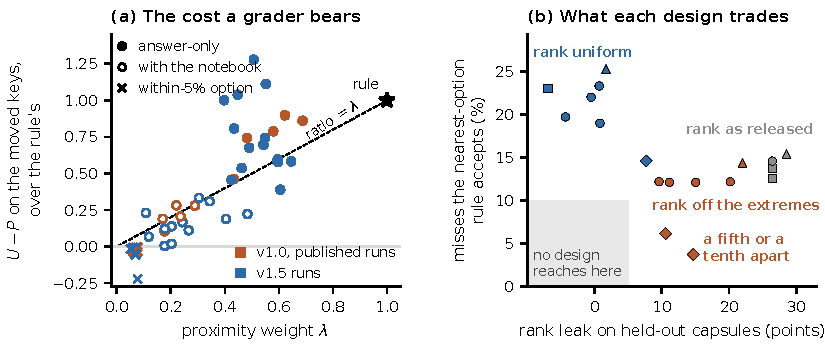
\includegraphics[width=\linewidth]{figures/cost.pdf}
\caption{\textbf{Who bears the cost of a hidden rank, and what each design of the options trades.} \textbf{(a)} Each
grading's $U-P$ on the moved keys divided by the nearest-option rule's on the same answers (star $=1$), against its
proximity weight $\lambda$ (\S\ref{sec:theory}); dashed: ratio $=\lambda$. \textbf{(b)} Each design of v1.5's numeric
options (\S\ref{sec:design}, Table~\ref{tab:design}): the rank leak, what a rank rule chosen on the other capsules
scores above chance on held-out ones, against the share of misses the nearest-option rule accepts. Colour: how the
key's rank is set; shape: how the distractors are made (squares $R$, $P$, $U$; circles redrawn as in $P$ and $U$;
diamonds a fifth or a tenth of the key apart; triangles other agents' wrong numbers). No design both leaks little and
accepts few misses.}
\label{fig:cost}
\end{figure}

On BixBench v1.5's $105$ four-option numeric items ($46$ capsules), the key's rank distribution is
$(p_1,\dots,p_4)=(12.4,51.4,29.5,6.7)\%$, far from uniform ($p=4\times10^{-8}$, treating each capsule's items as a
cluster; Figure~\ref{fig:overview}b). A rule that always selects the second-smallest option scores $+26.4$ $[+14.0,+38.6]$ points above chance, and
holding out each of the $46$ capsules in turn, the rank chosen on the other $45$ is always the second-smallest. On
v1.0's $159$ numeric items, the best rank rule scores $+5.8$ on the items it was chosen on but $-2.4$ when its rank is
chosen on the other capsules. The skew
arose in v1.5 (Table~\ref{tab:origin}): in the $24$ of v1.0's items whose distractors it rewrote, the key is second-smallest on $19$ ($79\%$, up from $29\%$ in v1.0). Of nine released multiple-choice datasets with
at least $20$ items whose options are all distinct numbers \citep{labbench,aquarat,medmcqa,medqa,mmlu,mmlupro,sciq},
BixBench's two included, five have a key rank that departs from uniform beyond chance when the items from one source
are treated as a cluster, and in four of these (v1.5, SciQ, MMLU-Pro and MMLU) a rank chosen on some clusters stays
above chance on the held-out ones (Table~\ref{tab:survey}). No model we tested is shown to use the rank
(Appendix~\ref{app:arms}). The leak threatens BixBench's no-data baseline, where a model above chance may be
reading the rank rather than recalling the answer, but not its scores with the data. Drawing the rank at random would close
the leak; we now ask what that costs.

\subsection{Hiding the rank costs a grader as far as it follows the nearest option}
\label{sec:cost}

\begin{figure}[t]
\centering
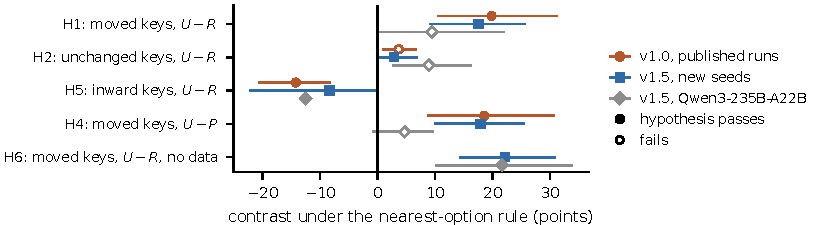
\includegraphics[width=\linewidth]{figures/test.pdf}
\caption{\textbf{The pre-specified test.} Each hypothesis's difference under the nearest-option rule, on the run
sets of the test, with the interval method fixed in advance: $U-R$ on a group of keys, $U-P$ for H4, and $U-R$ without
the data for H6 (not tested on the published runs). H2 on the published runs passes its stated criterion only by a
mean within $5$ points of zero and is counted as failed; Qwen3-235B-A22B's inward keys carry no interval, as no
interval reaches $95\%$ coverage on them. H3 passes on all three run sets.
Criteria and values: Table~\ref{tab:predictions}.}
\label{fig:test}
\end{figure}

Under the nearest-option rule, hiding the rank raises the share of the seven configurations' answers graded correct by
$+16.7$ $[+10.2,+23.0]$ points on the moved keys and by $+5.3$ $[+1.9,+8.6]$ over all numeric items
(Table~\ref{tab:cost}). Of the $47$ answers with the data that the rule accepts through $U$ but not through $R$, $46$
lie on the key's open side and $16$ are off by more than $100\%$ (Table~\ref{tab:mechanism}). The cost falls on misses,
so it shrinks as agents improve: over the nineteen run sets with the data, the rule's cost over all items falls as agents
land within $5\%$ of the key more often (rank correlation $-0.89$; Figure~\ref{fig:scaling}).

The other graders bear a share of the rule's cost that rises with their proximity weight (Figure~\ref{fig:cost}a). Answer-only graders follow
the nearest option most closely and bear most of the cost. Graders given BixBench's prompt and the notebook bear less,
and on the new seeds none of their costs is significant by the sign-flip test ($p=0.059$ to $0.861$). BixBench released its own grades only through $R$, so the cost its graders bear on the published runs' moved keys can only be
predicted from their proximity weights: $+6.9$ for gpt-4o's ($\lambda=0.24$) and $+20.1$ for Claude 3.5 Sonnet's
($\lambda=0.58$, within the answer-only graders' $0.48$ to $0.69$), though such predictions err by $3.9$ points on
average (Appendix~\ref{app:replication}). With the within-$5\%$ option, answer-only graders bear none of the
cost: hiding the rank changes what they accept on the moved keys by $-2.0$ to $-0.1$ points.

\paragraph{The pre-specified test.} Observation~\ref{obs:bracket} fixes the direction of H1, H3 and H5, so these
test only whether the effect is large enough to detect; all three pass on the published runs and the new seeds
(Figure~\ref{fig:test}). Of the two whose outcome Observation~\ref{obs:bracket} does not fix, H4 passes there too, and
H2 fails on the published runs, where $2.4$ of the unchanged keys' $+3.7$ points come from $11$ keys that $U$ moves
from one extreme to the other. H6 passes on both v1.5 run sets.
Qwen3-235B-A22B fails H1, H2 and H4 because redrawing the distractors farther from the key
(Appendix~\ref{app:options}) already accepts many of its near misses, whatever the key's rank
(Appendix~\ref{app:replication}). When the rule reads the last number, as the tolerance does, every hypothesis keeps its
verdict on every run set (Table~\ref{tab:lastnumber}).

\subsection{No design of the option values escapes the conflict}
\label{sec:design}

We rebuilt every numeric item's distractors under \emph{designs} an author could choose and regraded the same runs by
the rule and the four answer-only graders (Table~\ref{tab:design}, Appendix~\ref{app:design}, Figure~\ref{fig:cost}b).
A design sets the number of options $k$ ($4$ to $10$), the key's rank (as released at $k=4$, drawn from all $k$ ranks,
or drawn from the $k-2$ ranks off the extremes) and the distractors (spaced as in $P$ and $U$, a fixed fifth or tenth of
the key apart, or other agents' wrong numbers for the same question). Distractors taken from other agents' wrong
numbers leave the cost in place: drawing their key's rank uniformly rather than at its released rank raises the rule's
acceptance on the keys it moves to an extreme by $+24.1$ $[+16.3,+33.8]$ points on the published runs and $+18.8$
$[+11.3,+28.1]$ on v1.5. More options shrink both sides of the conflict: against a rank
kept off the extremes, a uniform rank costs the rule $11.1$ and $8.4$ points over all items at $k=4$ (v1.0 and v1.5)
and $6.1$ and $4.5$ at $k=8$, while a rank kept off the extremes reveals at least $25$ points at $k=4$ and $4.2$ at
$k=8$ (Tables~\ref{tab:design} and~\ref{tab:designpairs}). No design removes both the leak and the cost for a
grader that follows the nearest option. With the within-$5\%$ option the rank can be drawn uniformly without the cost,
since the grader applies the tolerance itself, but such graders reject $6.6$ to $17.9\%$ of correct answers
(Appendix~\ref{app:replication}).

\section{Discussion}
\label{sec:discussion}

\paragraph{Recommendations.} Other released datasets reveal the key's rank too (\S\ref{sec:leak}), and
Observation~\ref{obs:bracket} holds wherever free-text numeric answers are mapped to options by nearness, so these
recommendations apply beyond BixBench. \emph{Grade numeric answers by tolerance}, on a number extracted the same way for every
grading (Table~\ref{tab:extraction}). \emph{Report how many answers contain no number}, which a tolerance rejects and
forced choice can accept (\S\ref{sec:withdata}). \emph{Neither correct for guessing} (\S\ref{sec:guessing}) \emph{nor
compare forced-choice scores taken by graders that see different inputs} (\S\ref{sec:withdata}). \emph{If free-text
answers must be graded through options, add an option saying that no value is within the tolerance}, and report how many
correct answers the grader then rejects (\S\ref{sec:design}). \emph{For a no-data baseline}, where the model chooses among the
options itself, draw the key's rank uniformly and publish how often the key takes each rank (\S\ref{sec:leak}).

\paragraph{Limitations.} No human audited the accepted misses or the tolerance's verdicts. Our open-weight agents, run
at temperature $1.0$, are weak: with the data their number is within $5\%$ of the key on $2$ to $24\%$ of numeric
items (Figure~\ref{fig:scaling}); only the three current agents do better. Where the original graders cannot be run,
we substitute gpt-4o 2024-11-20 for 2024-08-06, and no model for the retired Claude 3.5 Sonnet; on the same misses, the
newer gpt-4o selects no option more than twice as often (Appendix~\ref{app:replication}). We chose the ten findings
corrected jointly after the v1.5 results. The plan of the pre-specified test was not registered publicly, so the evidence
that it preceded the analysis rests on GitHub's record of the push, archived with the code
(Appendix~\ref{app:replication}). We take the keys as released; on the $26$ numeric items whose keys
BixBench-Verified-50's experts re-checked, the excess and the rule's cost are about the same as on all items
(Table~\ref{tab:robust}). We do not show that forced
choice reverses any published ranking of agents. The study covers one benchmark's secondary metric, its
multiple-choice score, on v1.0's $159$ and v1.5's $105$ numeric items.

\section{Conclusion}
\label{sec:conclusion}

Forced choice accepts misses by where they fall among the options, and no correction for guessing removes this. Options
that hide the key's rank leave some keys extreme, where a grader that follows the nearest option accepts every miss
beyond the key on the open side, however far. A tolerance accepts none of these and reveals no rank.
The code, runs, grades and analyses at
\url{https://github.com/Vijayavallabh/forced-choice-tolerance} recompute every result without a GPU.

\begin{ack}
This work received no external funding, and the author declares no competing interests. Language-model assistance
was used in manuscript revision, code development and source checking; it does not constitute independent expert
validation.
\end{ack}

\bibliographystyle{plainnat}
\bibliography{refs}

\clearpage
\appendix

\section{Methods in detail}
\label{app:methods}

\subsection{Runs and gradings}
\label{app:withdata}

Our agent is BixBench's data-analysis agent at version 1.5.0 of its software, as the benchmark specifies, with its
system prompt, its prompt template for a free-text answer and its three tools (edit a notebook cell, list the working
directory, submit an answer). It takes at most $40$ steps at temperature $1.0$, with each capsule's files read-only in
our rebuild of BixBench's software container. Three open-weight model families ran in text, each served by the vLLM
inference server with 8-bit floating-point (FP8) weights and grading its own runs, as the published runs were graded
by the model that made them. ReAct runs use BixBench's ReAct agent at the versions the benchmark specifies. The
\emph{no-data} condition is the same agent with an empty working directory. Table~\ref{tab:settings} lists where our
runs depart from BixBench's agent. Each run is graded the two ways BixBench publishes: open-ended, by BixBench v1.5's
graders, and by its multiple-choice grader (prompts in Figure~\ref{fig:gradingprompts}). Table~\ref{tab:glossary}
defines the other graders, each at temperature $0$ and grading each run twice per option set, with the options in two
random orders.

\begin{table}[htbp]
\centering\footnotesize
\caption{The terms the paper uses.}
\label{tab:glossary}
\begin{tabularx}{\linewidth}{@{}lX@{}}
\toprule
term & meaning\\
\midrule
key; distractors & the correct option; the other options\\
numeric item & a question whose options are all numbers ($159$ in v1.0, $105$ in v1.5)\\
multiple-choice grader; forced, refusal & the model that maps an answer to an option, shown the notebook, the
question, the options and the answer; forced to choose, or offered BixBench's ``insufficient information'' option\\
selects no option & a forced grader's reply that names no option's letter (e.g.\ it says that none matches); BixBench
scores it wrong\\
tolerance; miss & the rule that accepts a submitted number (the last in the answer) within $5\%$ of the key; any
answer it rejects\\
capsule & a BixBench dataset with its questions\\
rank; bracketed, extreme, open side & the key's place among the sorted option values; a key with distractors on both
sides, or on one only; the side of an extreme key with none\\
published runs; current agents & BixBench's released v1.0 runs of gpt-4o and Claude 3.5 Sonnet; gpt-5.1, gpt-6-luna
and DeepSeek-V4-Pro run through BixBench's ReAct agent\\
configuration; run set & one agent model run one way: \emph{in text} (tool calls written as plain text) or
\emph{ReAct} (BixBench's own agent); one configuration's runs from one seed, or one published model's runs with or
without images\\
answer-only grader & shown the question, the options and the answer, not the notebook; the model server restricts its
reply to one option letter\\
letter-only grader & BixBench's prompt with the notebook, the reply restricted to an analysis and then one letter, so
it always selects an option\\
within-$5\%$ option & a fifth option stating that none of the others is within $5\%$ of the answer\\
excess & a grading's score minus the share of answers within $5\%$ of the key, in points\\
margin & accuracy above chance ($25\%$ with four options, $20\%$ with a refusal option), in points\\
corrected score & a forced score $S$ corrected for guessing (formula scoring), $(S-1/k)/(1-1/k)$
\citep{lordformula,frary}\\
rank rule; $p_j$ & a rule that always selects one rank, ignoring the question; the share of keys at rank $j$\\
nearest-option rule & selects, for a submitted number $a$, the option $v$ minimising $d(a,v)=|a-v|/(|a|+|v|)$, with
no model\\
$R$, $P$, $U$ & the released options; a rewrite preserving the key's rank; one drawing it uniformly\\
moved, inward, unchanged keys & keys $U$ moves from bracketed to extreme, from extreme to bracketed, or leaves
bracketed or extreme (possibly at another rank)\\
$U-P$; points & the cost of hiding the rank: the share of answers a grading accepts through $U$ minus that through
$P$; percentage points\\
proximity weight $\lambda$ & how closely a grader follows the nearest option, $(1-\delta)(qk-1)/(k-1)$, with $q$ the
share of its selections on misses that are the nearest option and $\delta$ the share of misses on which it selects
none; $1$ if it always selects the nearest option, $0$ if no more often than any other (Remark~\ref{rem:lambda})\\
sign-flip test & a test of a paired difference that flips the sign of each capsule's difference at random\\
new seeds & two further runs of each in-text configuration, made for the pre-specified test\\
$P'$, $U'$ & $P$ and $U$ with each new distractor written to the significant digits of the one it replaces\\
$\Gamma$; $\beta$ & the largest margin over chance that a grader seeing only the options (not the question) can
reach; the share of keys bracketed\\
uniform, middle designs & options whose key's rank is drawn from all $k$ ranks, or from the $k-2$ middle ones, so kept
off the extremes (Appendix~\ref{app:design})\\
agents' errors & distractors taken from other agents' wrong numbers on the same question\\
\bottomrule
\end{tabularx}
\end{table}

\begin{table}[htbp]
\centering\footnotesize
\caption{Where our runs depart from BixBench's own agent. A run cut short by one of our time limits was run
again from the start, so no kept run was cut short.}
\label{tab:settings}
\begin{tabularx}{\linewidth}{@{}>{\raggedright\arraybackslash}p{2.0cm}>{\raggedright\arraybackslash}X@{}}
\toprule
setting & our runs\\
\midrule
tool calls & in text: tool calls written as plain text; ReAct: BixBench's ReAct agent, whose tool-selection call
we start with the model family's own tool-call marker, because vLLM lacks the setting that forces that call to return
a tool\\
reasoning step & BixBench's reasoning step, the free-text call before each tool call, sends both Qwen families into a
repetition loop that runs to the $4{,}096$-token reply limit (all $183$ of Qwen2.5-72B's reasoning replies that reach
the limit and $2{,}090$ of Qwen3-30B-A3B's $2{,}276$); left as BixBench wrote it\\
network & none, where BixBench's agent had it ($8$ of the published runs' notebooks query the KEGG database online or
install an R package from CRAN); a failed connection or DNS lookup appears in $6$ to $22$ of each configuration's $105$
with-data runs on the numeric questions; it also appears in $16$ of gpt-5.1's $210$ and $12$ of gpt-6-luna's $105$,
none of which is within $5\%$ of the key\\
context window & $32{,}768$ tokens for Qwen2.5-72B and Qwen3-235B-A22B, $65{,}536$ for the other open models, $272{,}000$
for gpt-5.1 and gpt-6-luna, $128{,}000$ for DeepSeek-V4-Pro and Kimi-K3 (run, then left out;
Appendix~\ref{app:replication}); beyond it the older turns are cut to a few
hundred characters\\
notebook shown & $36{,}000$ characters for the open models, $300{,}000$ for gpt-5.1 and gpt-6-luna, $200{,}000$ for
DeepSeek-V4-Pro and Kimi-K3, cut by shortening the oldest cell outputs first, each cell output capped at
$6{,}000$\\
code execution & a persistent Jupyter kernel (the process that runs the notebook's code) runs each new cell alone and
stops it after $10$ minutes; BixBench's environment re-runs the whole notebook after every edit and attaches each plot
as an image, which our agent never sees\\
time limit & an hour per run; three hours for the new seeds and Qwen3-235B-A22B's later runs, and up to six for
Qwen3-30B-A3B\\
models & GLM-4.5-Air runs and grades with its built-in reasoning mode off; Qwen3-30B-A3B and Qwen3-235B-A22B are their Instruct-2507 releases\\
multiple-choice grader & reply capped at $1{,}536$ tokens ($4{,}096$ for GLM-4.5-Air), notebook at $60{,}000$ characters
($150{,}000$ for gemma-3-27b); gemma-3-27b grades Qwen3-30B-A3B's runs (Table~\ref{tab:withdata})\\
\bottomrule
\end{tabularx}
\end{table}

\begin{figure}[htbp]
\centering\footnotesize
\fbox{\begin{minipage}{0.95\linewidth}\raggedright\sloppy
\textbf{The grading prompts}, verbatim, with the prompts' own line breaks shown as line breaks. \texttt{\{\{question\}\}}
is BixBench's formatting of the question followed by its options as lettered lines (\texttt{A. \ldots}), shuffled
twice per run. With the refusal option, the fifth option is BixBench's ``Insufficient information to answer
the question''; with the within-$5\%$ option, it is ``None of the other options is within 5\% of the proposed
answer''. The multiple-choice grader's reply is read as the letter inside \texttt{<answer>} tags; the answer-only and
within-$5\%$ graders' reply is the single letter to which the model server restricts it. The letter-only grader uses
the multiple-choice grader's prompt (Table~\ref{tab:glossary}). Every grading is at temperature $0$.

\smallskip
\emph{Multiple-choice grader.} BixBench's \texttt{MCQ\_EVAL\_PROMPT}, with the run's notebook:

{\ttfamily\scriptsize First, carefully examine the following notebook:\par\smallskip
<notebook>\par \{\{notebook\}\}\par </notebook>\par\smallskip
Now, consider the following multiple-choice question:\par\smallskip
<question>\par \{\{question\}\}\par </question>\par\smallskip
For reference, this was an open response answer submitted to the question:\par\smallskip
<proposed\_answer>\par \{\{proposed\_answer\}\}\par </proposed\_answer>\par\smallskip
You are allowed to use the proposed answer as a reference, but you don't have to use it when selecting your final
answer.\par\smallskip
Your goal is to select the best answer for the MCQ based on the information provided in the notebook and any
associated images.\par
To ensure accuracy, please follow these steps:\par\smallskip
1. Carefully read and analyze the content of the notebook.\par
2. Review any associated images mentioned in the notebook.\par
3. Identify the relevant information from the notebook and images.\par
4. Consider each answer option carefully.\par
5. Select the best answer based on the available information.\par\smallskip
Before providing your final answer, wrap your analysis inside <question\_analysis> tags:\par
1. Quote the most relevant parts of the notebook for answering the question.\par
2. List arguments for and against each answer option.\par
3. Conclude with your chosen answer and a brief explanation.\par\smallskip
This process will help you arrive at the most accurate answer. It's OK for this section to be quite long.\par\smallskip
After completing your analysis, provide your final answer in the exact format shown below:\par\smallskip
<answer>A</answer>\par\smallskip
Remember:\par
- Only include the corresponding letter answers in your final output.\par
- DO NOT PROVIDE ANY ADDITIONAL EXPLANATIONS OR TEXT OUTSIDE OF THE LETTER.\par\smallskip
Please proceed with your analysis and answer selection.\par}

\smallskip
\emph{Answer-only grader.} The question and the answer as above, without the notebook, with an instruction to map
the answer to an option:

{\ttfamily\scriptsize Consider the following multiple-choice question:\par\smallskip
<question>\par \{\{question\}\}\par </question>\par\smallskip
This was an open response answer submitted to the question:\par\smallskip
<proposed\_answer>\par \{\{proposed\_answer\}\}\par </proposed\_answer>\par\smallskip
Map the proposed answer to the most appropriate answer option, and give the letter of that option.\par}

\smallskip
\emph{Within-$5\%$ option.} The answer-only prompt with its last line replaced by:

{\ttfamily\scriptsize Map the proposed answer to the answer option whose value is within 5\% of it. If no option's
value is within\par
5\% of the proposed answer, choose the option that says so. Give the letter of the option you choose.\par}

\smallskip
\emph{Open-ended grading.} BixBench v1.5's graders: an exact or partial string match, a range check, or a model
judge given BixBench's \texttt{OPEN\_ENDED\_GRADING\_PROMPT} (question, target answer, predicted answer; a reply of
\texttt{correct}, \texttt{incorrect} or \texttt{refused} in \texttt{<grade>} tags), as BixBench's grading code does.
\end{minipage}}
\caption{The grading prompts.}
\label{fig:gradingprompts}
\end{figure}

\subsection{The tolerance}
\label{app:reference}

The keys BixBench v1.5 writes as ranges have half-widths with lower and upper quartiles of $1.3$ and $11.5\%$. BixBench
v1.0's open-ended grader, whose verdicts were released with the runs, accepts $96\%$ of answers within $1\%$ of the
key, $40\%$ at $2$ to $5\%$ and $3\%$ at $10$ to $20\%$, so in effect it applies a tolerance
between $2$ and $10\%$. The v1.5 graders agree best with tolerances of $1$ and $2\%$ (Table~\ref{tab:tolerance}).
The tolerance reads the last number in an answer and, when the key is a percentage and the answer a fraction ($0.42$
for $42\%$), multiplies the answer by $100$. On the moved keys, no other way of reading the number gives a smaller $U-P$ than the pre-specified test's
(Table~\ref{tab:extraction}).

\begin{table}[htbp]
\centering\footnotesize\setlength{\tabcolsep}{4pt}
\caption{Tolerance rules against BixBench's own graders. \emph{v1.0}: BixBench v1.0's open-ended grader's verdicts on
gpt-4o's and Claude 3.5 Sonnet's $5{,}161$ with-data answers to numeric questions, with the answers it accepts
that a rule rejects, and the reverse; \emph{v1.5}: the v1.5 graders' verdicts on the seven configurations'
$735$ with-data answers to numeric questions. \emph{Key precision}: the answer, rounded to the precision at
which the key is written, equals the key. $\kappa$: Cohen's chance-corrected agreement.}
\label{tab:tolerance}
\begin{tabular}{lrrrr}
\toprule
& \multicolumn{3}{c}{v1.0 grader, published runs} & v1.5 graders\\
\cmidrule(lr){2-4}\cmidrule(lr){5-5}
rule & $\kappa$ & grader yes, rule no & grader no, rule yes & $\kappa$\\
\midrule
within 1\% & $0.87$ & $125$ & $27$ & $0.81$\\
within 2\% & $0.89$ & $78$ & $49$ & $0.81$\\
within 5\% & $0.90$ & $34$ & $86$ & $0.77$\\
within 10\% & $0.85$ & $26$ & $166$ & $0.71$\\
within 20\% & $0.74$ & $18$ & $366$ & $0.65$\\
key precision & $0.74$ & $241$ & $33$ & $0.78$\\
\bottomrule
\end{tabular}
\end{table}

\begin{table}[htbp]
\centering\footnotesize\setlength{\tabcolsep}{3pt}
\caption{How the nearest-option rule reads a number from an answer. \emph{Top}: with-data answers to numeric
questions, and the share, in per cent, that are empty, contain no number, are a number (what the pre-specified test's
rule reads), contain one number within text, or contain several. \emph{Bottom}: the rule's $U-P$, in points, on the
moved keys and over all numeric items, reading the number as the pre-specified test does (\emph{whole}), from the
last number in the answer as the tolerance does (\emph{last}), only in answers with exactly one number
(\emph{one}), and as in the test without the keys that are zero or negative (\emph{positive});
configurations pooled as in the test.}
\label{tab:extraction}
\begin{tabular}{lrrrrrr}
\toprule
& & \multicolumn{5}{c}{share of answers}\\
\cmidrule(lr){3-7}
answers & $n$ & empty & no number & a number & one in text & several\\
\midrule
v1.0, gpt-4o & $2{,}473$ & $2.1$ & $26.6$ & $57.6$ & $9.8$ & $3.9$\\
v1.0, Claude 3.5 Sonnet & $2{,}688$ & $0.5$ & $5.4$ & $91.0$ & $2.5$ & $0.6$\\
v1.5, seven configurations & $735$ & $13.1$ & $11.0$ & $59.9$ & $8.7$ & $7.3$\\
v1.5, new seeds & $630$ & $7.9$ & $7.8$ & $68.1$ & $11.1$ & $5.1$\\
v1.5, Qwen3-235B-A22B & $210$ & $9.5$ & $15.2$ & $73.8$ & $0.5$ & $1.0$\\
\midrule
& \multicolumn{4}{c}{moved keys} & \multicolumn{2}{c}{all items}\\
\cmidrule(lr){2-5}\cmidrule(lr){6-7}
$U-P$ & whole & last & one & positive & whole & last\\
\midrule
v1.0, published & $+18.6$ & $+21.9$ & $+25.8$ & $+19.6$ & $+3.4$ & $+4.6$\\
v1.5, seven configurations & $+16.7$ & $+24.8$ & $+30.8$ & $+18.2$ & $+5.3$ & $+8.3$\\
v1.5, new seeds & $+17.9$ & $+24.2$ & $+28.2$ & $+19.5$ & $+6.6$ & $+8.7$\\
v1.5, Qwen3-235B-A22B & $+4.7$ & $+4.7$ & $+8.3$ & $+5.1$ & $+1.2$ & $+1.2$\\
\bottomrule
\end{tabular}
\end{table}

\subsection{Option sets}
\label{app:options}

$P$ and $U$ keep each item's question and key and replace its three distractors with values from one generator,
which is given a rank for the key: the released rank for $P$, and a rank drawn uniformly from the four for $U$. The generator never
sees the question, the runs or any grading. When the four released values share the key's sign, the $j$-th new
distractor on each side of the key $y$, counting outward, lies at $y(1+sju)$ or $y/(1+sju)$, where $u$ is drawn
uniformly from $[0.6,1.4]$ and $s$ is the released distractors' mean relative distance from the key (raised to $0.05$
if smaller); otherwise at $y\pm Dju$, with $D$ their mean absolute distance. Each new value is written in the notation of the distractor it
replaces. A draw that makes two options equal, changes a value's sign or moves the key off its rank is redrawn with a
wider spread, up to $24$ times. If every redraw fails, $U$ takes another rank ($3$ of v1.5's $105$ items and $10$ of v1.0's
$159$) and $P$ leaves the item out ($1$ of v1.0's). Each rewrite is one draw at a fixed seed. The generator's nearest
distractor lies farther from the key than in $R$ (a median $d$ of $0.185$ in $P$ and $0.188$ in $U$, against
$0.142$), so $P-R$ is not zero. As $P$ and $U$ share the redrawing, $U-P$ isolates the rank.

In $P$ and $U$ the key stands out by its significant digits. The digit-matched $P'$ and $U'$ remove that cue: each new
value also takes the significant digits of the distractor it replaces, assigned in order of size. A rule that
selects the option with the fewest significant digits is then correct on $25.3$ and $25.5\%$ of v1.5's $P'$ and $U'$,
against $25.0\%$ on $R$ and $31.7$ and $31.9\%$ on $P$ and $U$. For every set of runs but DeepSeek-V4-Pro's, the
nearest-option rule's $U'-P'$ lies within $2.9$ points of its $U-P$ on the moved keys, the unchanged keys and all items;
DeepSeek-V4-Pro's cost rests on two to four answers and falls to zero.

\subsection{Statistics}
\label{app:stats}

Every interval is a percentile bootstrap over capsules: we resample the capsules with replacement and read the
interval from the percentiles of the resampled estimates. Each is read at the nominal level that covers the
true value $95\%$ of the time (\S\ref{sec:stats}), except a \emph{plain} $95\%$ interval, the uncorrected range from
the $2.5$th to the $97.5$th percentile.
For a margin or a difference over all of a release's items, the level comes from data simulated with each condition's
own capsule sizes and spread of accuracy between capsules (a beta-binomial distribution matched to the observed mean
and variance): v1.5's $46$ capsules, of unequal size, carry as much information as $29.6$ equal ones (Kish's effective
sample size), and its margins and differences are read at $96.75$ and $96.0\%$. For a paired difference per question,
and for any subset of a release's items, a nested resampling (a double bootstrap) sets the level: the lowest, on a grid from $80$ to $99.995\%$, at which the intervals of at least $2{,}000$ resamples of the
capsules hold the full sample's estimate $95\%$ of the time. Where no level on the grid does, the estimate is given
without an interval and marked $^{\ddagger}$. When a paired difference is exactly zero on most capsules, a resample
can draw only those capsules and give exactly zero; when that is likelier than the interval's tail, that end of the
interval is set to zero, which is why several intervals end at $+0.0$. The sign-flip test (\S\ref{sec:stats}) compares a paired
difference's mean with the means under flipped signs, over every pattern up to $20$ capsules and $200{,}000$ random patterns beyond. It assumes only that each capsule's difference is
symmetric about the true value; turned into an interval, it contained the true value in $197$ of $200$ simulated
data sets built like the moved keys.

We correct ten headline findings jointly (Table~\ref{tab:claims}): each is read at the level that attains
$1-0.05/10=99.5\%$ coverage on its own data (a Bonferroni correction), so the findings that survive hold
together; a finding with several parts survives only if every part does. We chose the
ten after seeing the results, so the correction guards against chance among them but not against how they were
chosen. The pre-specified test is not among them.

\FloatBarrier
\section{Proofs}
\label{app:theory}

\paragraph{What the options alone reveal.} An item presents a set $V$ of $k$ options, one of which is the key $Y$. A
grader that sees only $V$ (neither the question nor the data) can exceed chance by at most
\begin{equation}
\Gamma \;=\; \mathbb{E}_V\Big[\max_{v\in V}\Pr(Y=v\mid V)\Big]-\tfrac1k ,
\label{eq:gamma}
\end{equation}
the best margin that a choices-only baseline \citep{choicesonly}, which answers from the options alone, could reach
on unlimited items generated the same way.
$\Gamma$ depends on the process that generated the options, so it cannot be computed for a released dataset, but the rank rules of \S\ref{sec:theory} bound it from
below. A margin over chance shows that the options reveal the key, but a score at chance does not show that they
conceal it:

\begin{lemma}[when the options reveal nothing]
\label{lem:flat}
$\Gamma=0$ if and only if $\Pr(Y=v\mid V)=\tfrac1k$ for almost every presented $V$, and then every grader
that sees only the options is correct with probability exactly $\tfrac1k$, whatever statistic of the options
it uses.
\end{lemma}

\paragraph{Proof of Lemma~\ref{lem:flat}.} $\max_{v\in V}\Pr(Y=v\mid V)\ge\frac1k\sum_{v\in
V}\Pr(Y=v\mid V)=\frac1k$ for every $V$, so $\Gamma\ge0$ always and $\Gamma=0$ forces
$\max_{v}\Pr(Y=v\mid V)=\frac1k$ with probability one, which for $k$ non-negative numbers summing to one
means all of them equal $\frac1k$. Conversely, if every option is equally likely to be the key given $V$, the maximum
is $\frac1k$ on every $V$. A grader that sees only $V$ picks $\pi(V)\in V$ by any rule and any randomness, and
$\Pr[\pi(V)=Y]=\mathbb{E}_V\Pr(Y=\pi(V)\mid V)=\frac1k$; the statistic it uses never enters.

\paragraph{The rank rule's floor.} A bracketed key has one of the $k-2$ middle ranks, so if a share $\beta$ of a
dataset's keys are bracketed, $\sum_{j=2}^{k-1}p_j=\beta$ and the largest of those $k-2$ terms is at least their mean,
$\beta/(k-2)$. The rule that always selects that rank uses only $V$ and scores $p_j$, and no rule using
only $V$ scores more than $\mathbb{E}_V[\max_v\Pr(Y=v\mid V)]$, so $\Gamma\ge\max_jp_j-\tfrac1k\ge
\beta/(k-2)-\tfrac1k$ (Table~\ref{tab:survey} gives both bounds for nine datasets). A rank uniform over the $k-2$ middle
ranks makes $p_j=1/(k-2)$ for each middle $j$, so $\Gamma\ge1/(k-2)-1/k=2/(k(k-2))$; a rank uniform over all $k$
makes every $p_j=1/k$ and leaves $2/k$ of the keys at the extremes.

\paragraph{Proof of Observation~\ref{obs:bracket}.} For $a,v$ of the same sign write $r=|a|/|v|$: $d(a,v)=|r-1|/(r+1)=
\tanh(|\log r|/2)$, increasing in $|\log|a|-\log|v||$, and $d(a,v)=1$ when the signs differ or one of them is
zero. Let the key $y\ne0$ be the largest in magnitude among the options of its sign, and $a$ an answer of that
sign with $|a|>|y|$. Every other option $v$ of that sign has $|v|<|y|<|a|$, so $\log|y|$ lies between $\log|v|$
and $\log|a|$, $|\log|a|-\log|y||<|\log|a|-\log|v||$ and $d(a,y)<d(a,v)$; every option of the other sign, or
zero, has $d(a,v)=1>d(a,y)$. The smallest-magnitude case is symmetric, with $|a|<|y|<|v|$. For a positive key
largest in magnitude means largest in value; for a negative key it means smallest in value. For $a$ and $v$ of the
key's sign, $d(a,y)<d(a,v)$ exactly when $\log|a|$ lies on $y$'s side of the midpoint of $\log|y|$ and $\log|v|$, the
logarithm of the geometric mean $\sqrt{|y||v|}$. With the key's nearest options of its sign at magnitudes
$|y|/\rho_-$ and $|y|\rho_+$, a miss of its sign is therefore nearest the key exactly when
$|y|/\sqrt{\rho_-}<|a|<|y|\sqrt{\rho_+}$. An extreme key has no such neighbour on its open side, and every answer of
its sign beyond it is nearest it. The part on extreme keys holds for any distance that grows with the gap between
two numbers; the bounds in $\sqrt{\rho_\pm}$ are specific to $d$. Under $d$, a key is extreme when it is the smallest
or largest in magnitude among the options of its sign. This differs from its rank among all the values when zero or a
negative option lies below a positive key ($2$ of v1.5's $105$ released keys, $2$ of v1.0's $159$) and when the key is
zero ($4$ and $2$), since zero is at distance $1$ from every nonzero answer. The pre-specified test uses the key's rank
among all the values, as its plan specified, and scores an answer at distance $1$ from every option as a tie among all
the options, worth the expected score of a random tie-break.

\begin{remark}
\label{rem:lambda}
Let a forced grader, on a miss whose number has a single nearest option, select no option with probability
$\delta$ and, when it selects one, the nearest option with probability $q$ and each other option with probability
$(1-q)/(k-1)$, whatever the options. Then a change of options that makes the key the nearest option for a share
$\Delta$ of the misses
raises the share it accepts by $\lambda\Delta$, where $\lambda=(1-\delta)(qk-1)/(k-1)$.
\end{remark}

\paragraph{Derivation of Remark~\ref{rem:lambda}.} On a miss whose number has a single nearest option the grader accepts with
probability $(1-\delta)q$ if that option is the key and $(1-\delta)(1-q)/(k-1)$ if it is not. A change of options
that moves a share $\Delta$ of these misses from the second case to the first raises acceptance by
$\Delta(1-\delta)\big(q-(1-q)/(k-1)\big)=\lambda\Delta$; misses whose nearest option is the key under both option
sets, or under neither, contribute nothing.

\paragraph{Shuffling the displayed order does not hide the rank.} What must be random is which value is the key, not
the order in which the options are shown, so shuffling that order, as BixBench does, does not give $\Gamma=0$.
Exchangeability suffices: if the $k$ values
$(\text{key},\text{distractor}_1,\dots,\text{distractor}_{k-1})$ are exchangeable, that is, their joint distribution
is unchanged by any reordering, then the key is equally likely to be any option, so $\Gamma=0$. The converse fails:
draw any $k$ values, make one of them the key at random, and list the other $k-1$ in increasing order. Every option is
then equally likely to be the key and $\Gamma=0$, yet swapping two distractors gives orders that never occur, so the
values are not exchangeable.

\FloatBarrier
\section{Results in detail}
\label{app:results}

Eight of the ten headline findings survive the joint correction of Appendix~\ref{app:stats}
(Table~\ref{tab:claims}).

\begin{table}[htbp]
\centering\footnotesize\setlength{\tabcolsep}{4pt}
\caption{The paper's ten headline findings, corrected jointly. Each row gives the estimate, in points above the
stated comparison; its interval as the paper states it elsewhere, at the level that attains $95\%$ coverage; and the
jointly corrected interval (\emph{joint}), at the level that attains $1-0.05/10$ coverage on each data set's own
capsules, calibrated by simulation or, for the paired differences, by the double bootstrap (Appendix~\ref{app:stats}).
Rows $1$, $2$, $3$, $4$--$5$, $6$--$7$, $8$--$9$, $10$, $11$--$13$, $14$ and $15$--$17$ are the ten findings. Rows
$4$--$5$ must fall below the value a model would show if its whole margin came from choosing the second-smallest option
(Table~\ref{tab:attribution}), for both models; the excess over the tolerance and the acceptance of misses nearest the
key must hold for both published models, the current agents' excess for all three agents, and the graders' $U-P$ on
the published runs for all three graders. Every finding holds with its own $95\%$ interval. $^{\times}$Does not hold
once the ten are corrected jointly.}
\label{tab:claims}
\begin{tabularx}{\linewidth}{@{}>{\raggedright\arraybackslash}Xlrrr@{}}
\toprule
Finding & Data; compared with & Estimate & $95\%$ & Joint\\
\midrule
A rule that ignores the question selects the second-smallest option & v1.5, $105$ numeric; chance & $+26.4$ & $[+14.0,+38.6]$ & $[+9.4,+42.8]$\\
BixBench's released forced-choice run without the data, gpt-4o & v1.5, $205$; chance & $+11.1$ & $[+3.8,+18.8]$ & $[+0.4,+22.8]$\\
The same, Claude 3.5 Sonnet & v1.5, $205$; chance & $+9.1$ & $[+2.5,+16.4]$ & $[-0.2,+20.1]$$^{\times}$\\
Accuracy where the key is second-smallest minus elsewhere, gpt-4o & v1.5, $105$ numeric; below $+45.9$ & $-7.8$ & $[-27.1,+12.9]$ & $[-34.0,+20.5]$\\
The same, Claude 3.5 Sonnet & v1.5, $105$ numeric; below $+35.1$ & $-13.4$ & $[-36.2,+11.3]$ & $[-43.1,+20.7]$\\
BixBench's forced-choice grading of $R$, gpt-4o's published runs & v1.0, $159$ numeric; within $5\%$ & $+19.2$ & $[+15.5,+23.4]$ & $[+13.8,+25.5]$\\
The same, Claude 3.5 Sonnet's & v1.0, $159$ numeric; within $5\%$ & $+21.0$ & $[+17.3,+25.0]$ & $[+14.9,+28.1]$\\
Its acceptance of misses nearest the key, gpt-4o's published runs & v1.0; misses nearest another & $+31.2$ & $[+17.1,+43.3]$ & $[+10.4,+49.0]$\\
The same, Claude 3.5 Sonnet's & v1.0; misses nearest another & $+56.9$ & $[+47.0,+66.8]$ & $[+42.1,+71.3]$\\
The tolerance above the forced-choice score corrected for guessing, seven configurations & v1.5, $105$ numeric; the correction & $+10.6$ & $[+6.8,+14.3]$ & $[+4.8,+16.0]$\\
Forced-choice grading by gpt-4o, gpt-5.1's runs & v1.5, $105$ numeric; within $5\%$ & $+10.0$ & $[+3.5,+16.6]$ & $[+1.2,+18.8]$\\
The same, gpt-6-luna's & v1.5, $105$ numeric; within $5\%$ & $+11.0$ & $[+3.6,+18.5]$ & $[-1.1,+24.3]$$^{\times}$\\
The same, DeepSeek-V4-Pro's & v1.5, $105$ numeric; within $5\%$ & $+11.9$ & $[+4.6,+19.4]$ & $[+0.6,+23.4]$\\
With the data, $U-P$ on the moved keys, nearest-option rule & $37$ items, $7$ configurations & $+16.7$ & $[+10.2,+23.0]$ & $[+7.5,+26.9]$\\
With the data, $U-P$ on the moved keys, Qwen2.5-72B grading BixBench's published runs & v1.0, $40$ items & $+14.4$ & $[+7.0,+22.2]$ & $[+3.8,+27.1]$\\
The same, gemma-3-27b grading them & v1.0, $40$ items & $+8.7$ & $[+4.3,+14.0]$ & $[+2.1,+17.7]$\\
The same, Llama-3.3-70B grading them & v1.0, $40$ items & $+8.8$ & $[+3.7,+14.1]$ & $[+0.7,+18.5]$\\
\bottomrule
\end{tabularx}
\end{table}

\subsection{What forced choice accepts}
\label{app:excess}

Table~\ref{tab:reference} recomputes Table~\ref{tab:released}'s excess against four other references,
Table~\ref{tab:allq} extends it to every question, and Table~\ref{tab:restated} restates every tolerance-dependent
result at $1$, $2$ and $10\%$. On the questions whose options are not numbers, the published grades exceed the
open-ended ones by more than a random choice on every miss would add.

\begin{table}[htbp]
\centering\scriptsize\setlength{\tabcolsep}{2pt}
\caption{\textbf{The forced-choice excess against other references.} BixBench's multiple-choice grading of the released options, with its prompt and the notebook, minus each reference,
in points, on the with-data runs of Table~\ref{tab:released}. The references are the $5\%$ tolerance on the last number
in the answer (as in Table~\ref{tab:released}); BixBench's own open-ended grading of the same runs, which reads the whole
answer (the v1.0 grader on the published runs, the v1.5 graders on the seven configurations); the $5\%$ tolerance on any
number in the answer; the tolerance without the items whose key is a p-value ($19$ of v1.0's $159$, $8$ of v1.5's $105$); and the
tolerance with those keys graded within a factor of ten. Intervals as in Table~\ref{tab:released}.}
\label{tab:reference}
\resizebox{\linewidth}{!}{\begin{tabular}{llrrrrr}
\toprule
runs & grading & tolerance & open-ended grading & any number & no p-value keys & p-values within $\times10$\\
\midrule
v1.0, gpt-4o & forced & $+19.2$ {\scriptsize$[+15.5,+23.4]$} & $+20.4$ {\scriptsize$[+17.1,+23.9]$} & $+19.1$ {\scriptsize$[+15.4,+23.3]$} & $+19.5$ {\scriptsize$[+15.5,+23.8]$} & $+17.5$ {\scriptsize$[+13.6,+21.6]$}\\
 & with refusal & $+0.7$ {\scriptsize$[-0.4,+1.9]$} & $+1.9$ {\scriptsize$[+0.4,+4.2]$} & $+0.6$ {\scriptsize$[-0.5,+1.9]$} & $+1.0$ {\scriptsize$[-0.2,+2.4]$} & $-1.0$ {\scriptsize$[-3.0,+0.8]$}\\
v1.0, Claude 3.5 Sonnet & forced & $+21.0$ {\scriptsize$[+17.3,+25.0]$} & $+21.7$ {\scriptsize$[+18.1,+25.5]$} & $+21.0$ {\scriptsize$[+17.4,+24.9]$} & $+21.6$ {\scriptsize$[+17.2,+26.6]$} & $+19.1$ {\scriptsize$[+14.9,+23.5]$}\\
 & with refusal & $+3.1$ {\scriptsize$[-0.3,+9.6]$} & $+3.8$ {\scriptsize$[+1.0,+7.8]$} & $+3.1$ {\scriptsize$[-0.4,+9.2]$} & $+3.4$ {\scriptsize$[-0.6,+11.7]$} & $+1.2$ {\scriptsize$[-2.6,+5.5]$}\\
v1.5, seven configurations & forced & $+14.6$ {\scriptsize$[+12.0,+17.2]$} & $+14.1$ {\scriptsize$[+10.8,+17.3]$} & $+13.9$ {\scriptsize$[+11.5,+16.3]$} & $+14.0$ {\scriptsize$[+11.1,+16.7]$} & $+14.4$ {\scriptsize$[+11.4,+17.1]$}\\
 & with refusal & $+1.3$ {\scriptsize$[-0.7,+3.3]$} & $+0.7$ {\scriptsize$[-2.2,+3.5]$} & $+0.6$ {\scriptsize$[-1.1,+2.3]$} & $+1.1$ {\scriptsize$[-1.1,+3.2]$} & $+1.0$ {\scriptsize$[-1.0,+3.1]$}\\
\bottomrule
\end{tabular}}
\end{table}

\begin{table}[htbp]
\centering\scriptsize\setlength{\tabcolsep}{2pt}
\caption{\textbf{What grading through options adds over every question.} Each grading's score minus BixBench's open-ended grade of the same runs, in points, on the numeric questions, the
others and all. Parentheses give what a random choice among the four options on every miss would add (a quarter of the
misses); brackets give a plain $95\%$ interval over capsules, on all questions.
\emph{Published}: BixBench's own forced grades, with the notebook; \emph{own model}: each configuration's own
model, with the notebook; \emph{answer-only} as in Table~\ref{tab:glossary}; \emph{refused}: the share of
gradings selecting the refusal option, in per cent. Each question's runs are averaged within a model, then over the models. v1.0: $296$ questions, $159$ of them numeric ($289$ and $158$ with gpt-4o's runs); v1.5: $205$, $105$
numeric.}
\label{tab:allq}
\resizebox{\linewidth}{!}{\begin{tabular}{llrrrr}
\toprule
runs & grading & numeric & other & all & refused\\
\midrule
v1.0, gpt-4o & published & $+20.4$ {\scriptsize$(+22.4)$} & $+29.0$ {\scriptsize$(+21.9)$} & $+24.3$ {\scriptsize$[+21.2,+27.5]$} {\scriptsize$(+22.2)$} & --\\
 & gpt-4o, answer-only & $+24.2$ {\scriptsize$(+22.4)$} & $+30.8$ {\scriptsize$(+21.9)$} & $+27.2$ {\scriptsize$[+24.0,+30.6]$} {\scriptsize$(+22.2)$} & --\\
 & gemma-3-27b, answer-only & $+23.1$ {\scriptsize$(+22.4)$} & $+27.2$ {\scriptsize$(+21.9)$} & $+25.0$ {\scriptsize$[+21.5,+28.6]$} {\scriptsize$(+22.2)$} & --\\
 & Qwen2.5-72B, answer-only & $+25.2$ {\scriptsize$(+22.4)$} & $+32.2$ {\scriptsize$(+21.9)$} & $+28.4$ {\scriptsize$[+24.4,+32.4]$} {\scriptsize$(+22.2)$} & --\\
 & Llama-3.3-70B, answer-only & $+27.3$ {\scriptsize$(+22.4)$} & $+28.2$ {\scriptsize$(+21.9)$} & $+27.7$ {\scriptsize$[+24.2,+31.3]$} {\scriptsize$(+22.2)$} & --\\
 & gpt-4o, answer-only, refusal & $+2.0$ {\scriptsize$(+22.4)$} & $+8.1$ {\scriptsize$(+21.9)$} & $+4.8$ {\scriptsize$[+2.9,+6.8]$} {\scriptsize$(+22.2)$} & $74$\\
 & gemma-3-27b, answer-only, refusal & $+3.9$ {\scriptsize$(+22.4)$} & $+9.0$ {\scriptsize$(+21.9)$} & $+6.2$ {\scriptsize$[+4.2,+8.4]$} {\scriptsize$(+22.2)$} & $69$\\
v1.0, Claude 3.5 Sonnet & published & $+21.7$ {\scriptsize$(+21.3)$} & $+20.2$ {\scriptsize$(+19.4)$} & $+21.0$ {\scriptsize$[+18.6,+23.6]$} {\scriptsize$(+20.4)$} & --\\
 & gpt-4o, answer-only & $+21.4$ {\scriptsize$(+21.3)$} & $+21.9$ {\scriptsize$(+19.4)$} & $+21.6$ {\scriptsize$[+19.1,+24.3]$} {\scriptsize$(+20.4)$} & --\\
 & gemma-3-27b, answer-only & $+20.7$ {\scriptsize$(+21.3)$} & $+19.2$ {\scriptsize$(+19.4)$} & $+20.0$ {\scriptsize$[+17.2,+23.1]$} {\scriptsize$(+20.4)$} & --\\
 & Qwen2.5-72B, answer-only & $+23.6$ {\scriptsize$(+21.3)$} & $+24.0$ {\scriptsize$(+19.4)$} & $+23.8$ {\scriptsize$[+20.4,+27.2]$} {\scriptsize$(+20.4)$} & --\\
 & Llama-3.3-70B, answer-only & $+23.6$ {\scriptsize$(+21.3)$} & $+19.9$ {\scriptsize$(+19.4)$} & $+21.9$ {\scriptsize$[+18.8,+25.1]$} {\scriptsize$(+20.4)$} & --\\
 & gpt-4o, answer-only, refusal & $+0.4$ {\scriptsize$(+21.3)$} & $+5.4$ {\scriptsize$(+19.4)$} & $+2.8$ {\scriptsize$[+1.2,+4.4]$} {\scriptsize$(+20.4)$} & $63$\\
 & gemma-3-27b, answer-only, refusal & $+3.8$ {\scriptsize$(+21.3)$} & $+7.8$ {\scriptsize$(+19.4)$} & $+5.6$ {\scriptsize$[+3.9,+7.6]$} {\scriptsize$(+20.4)$} & $54$\\
v1.5, seven configurations & own model & $+14.1$ {\scriptsize$(+22.4)$} & $+16.2$ {\scriptsize$(+20.8)$} & $+15.1$ {\scriptsize$[+12.9,+17.4]$} {\scriptsize$(+21.6)$} & --\\
 & gpt-4o, answer-only & $+15.6$ {\scriptsize$(+22.4)$} & $+19.0$ {\scriptsize$(+20.8)$} & $+17.3$ {\scriptsize$[+14.5,+20.1]$} {\scriptsize$(+21.6)$} & --\\
 & gemma-3-27b, answer-only & $+12.8$ {\scriptsize$(+22.4)$} & $+18.9$ {\scriptsize$(+20.8)$} & $+15.7$ {\scriptsize$[+13.4,+18.1]$} {\scriptsize$(+21.6)$} & --\\
 & Qwen2.5-72B, answer-only & $+17.6$ {\scriptsize$(+22.4)$} & $+17.3$ {\scriptsize$(+20.8)$} & $+17.4$ {\scriptsize$[+14.1,+20.9]$} {\scriptsize$(+21.6)$} & --\\
 & Llama-3.3-70B, answer-only & $+12.9$ {\scriptsize$(+22.4)$} & $+16.9$ {\scriptsize$(+20.8)$} & $+14.8$ {\scriptsize$[+12.1,+17.7]$} {\scriptsize$(+21.6)$} & --\\
 & gpt-4o, answer-only, refusal & $-0.5$ {\scriptsize$(+22.4)$} & $+3.8$ {\scriptsize$(+20.8)$} & $+1.6$ {\scriptsize$[+0.1,+3.1]$} {\scriptsize$(+21.6)$} & $70$\\
 & gemma-3-27b, answer-only, refusal & $+0.7$ {\scriptsize$(+22.4)$} & $+5.7$ {\scriptsize$(+20.8)$} & $+3.2$ {\scriptsize$[+1.6,+4.6]$} {\scriptsize$(+21.6)$} & $61$\\
v1.5, gpt-5.1 & gpt-4o & $+15.2$ {\scriptsize$(+19.4)$} & $+15.2$ {\scriptsize$(+17.6)$} & $+15.2$ {\scriptsize$[+11.5,+19.2]$} {\scriptsize$(+18.5)$} & --\\
 & gpt-4o, answer-only & $+23.8$ {\scriptsize$(+19.4)$} & $+19.5$ {\scriptsize$(+17.6)$} & $+21.7$ {\scriptsize$[+16.3,+27.6]$} {\scriptsize$(+18.5)$} & --\\
 & gemma-3-27b, answer-only & $+23.8$ {\scriptsize$(+19.4)$} & $+18.8$ {\scriptsize$(+17.6)$} & $+21.3$ {\scriptsize$[+16.6,+26.5]$} {\scriptsize$(+18.5)$} & --\\
 & gpt-4o, answer-only, refusal & $+5.7$ {\scriptsize$(+19.4)$} & $+2.0$ {\scriptsize$(+17.6)$} & $+3.9$ {\scriptsize$[+0.8,+7.4]$} {\scriptsize$(+18.5)$} & $61$\\
 & gemma-3-27b, answer-only, refusal & $+8.3$ {\scriptsize$(+19.4)$} & $+4.0$ {\scriptsize$(+17.6)$} & $+6.2$ {\scriptsize$[+2.4,+10.6]$} {\scriptsize$(+18.5)$} & $53$\\
\bottomrule
\end{tabular}}
\end{table}

\begin{table}[htbp]
\centering\scriptsize\setlength{\tabcolsep}{3pt}
\caption{The paper's tolerance-dependent results at four tolerances. From the top: the answers given without
options and without the data (Table~\ref{tab:arms}), regraded with no model (any number in the reply within the
tolerance); Qwen2.5-72B's with-data runs (Appendix~\ref{app:withdata}; intervals paired over $46$ capsules at $96\%$);
the best of six open-weight models asked for a number without options (Appendix~\ref{app:arms}), counting any number in
the reply; BixBench's gradings of Table~\ref{tab:released} minus the tolerance (intervals as in
Table~\ref{tab:released}); and the share of misses that the nearest-option rule accepts through $R$ and $U$.
Table~\ref{tab:mechanism}'s distance bins are not restated: they describe how far accepted answers lie from the key and
give no verdict.}
\label{tab:restated}
\resizebox{\linewidth}{!}{\begin{tabular}{lrrrr}
\toprule
& $1\%$ & $2\%$ & $5\%$ & $10\%$\\
\midrule
Table~\ref{tab:arms}, v1.5, gpt-4o & $0.6$ & $0.6$ & $1.2$ & $1.2$\\
Table~\ref{tab:arms}, v1.5, Claude 3.5 & $1.8$ & $1.8$ & $2.4$ & $3.0$\\
Table~\ref{tab:arms}, v1.0, gpt-4o & $3.1$ & $3.1$ & $4.3$ & $4.9$\\
Table~\ref{tab:arms}, v1.0, Claude 3.5 & $4.3$ & $4.3$ & $6.1$ & $8.0$\\
Qwen2.5-72B within, with the data & $13.3$ & $13.3$ & $14.3$ & $14.3$\\
\quad without it & $1.0$ & $1.0$ & $1.0$ & $2.9$\\
\quad with $-$ without & $+12.4$ {\scriptsize$[+4.9,+22.2]$} & $+12.4$ {\scriptsize$[+4.9,+22.2]$} & $+13.3$ {\scriptsize$[+5.6,+23.5]$} & $+11.4$ {\scriptsize$[+2.9,+22.3]$}\\
\quad lead over Llama-3.3-70B & $+8.6$ {\scriptsize$[+0.0,+18.6]$} & $+8.6$ {\scriptsize$[+0.0,+18.6]$} & $+9.5$ {\scriptsize$[+0.9,+20.0]$} & $+4.8$ {\scriptsize$[-4.3,+15.3]$}\\
\quad lead over gemma-3-27b & $+11.4$ {\scriptsize$[+4.1,+21.3]$} & $+11.4$ {\scriptsize$[+4.1,+21.3]$} & $+10.5$ {\scriptsize$[+2.0,+21.4]$} & $+9.5$ {\scriptsize$[+0.9,+20.6]$}\\
open-weight models, any number, best & $3.8$ & $3.8$ & $3.8$ & $4.8$\\
Table~\ref{tab:released}, gpt-4o, forced & $+21.2$ {\scriptsize$[+17.4,+25.3]$} & $+20.1$ {\scriptsize$[+16.5,+24.0]$} & $+19.2$ {\scriptsize$[+15.5,+23.4]$} & $+18.2$ {\scriptsize$[+14.6,+22.1]$}\\
\quad Claude 3.5 Sonnet, forced & $+24.3$ {\scriptsize$[+20.6,+28.1]$} & $+23.0$ {\scriptsize$[+19.4,+26.8]$} & $+21.0$ {\scriptsize$[+17.3,+25.0]$} & $+18.8$ {\scriptsize$[+14.8,+23.1]$}\\
\quad gpt-4o, with refusal & $+2.7$ {\scriptsize$[+0.7,+5.5]$} & $+1.6$ {\scriptsize$[+0.4,+2.9]$} & $+0.7$ {\scriptsize$[-0.4,+1.9]$} & $-0.4$ {\scriptsize$[-1.6,+0.8]$}\\
\quad Claude 3.5 Sonnet, with refusal & $+6.3$ {\scriptsize$[+2.8,+10.7]$} & $+5.1$ {\scriptsize$[+1.8,+9.7]$} & $+3.1$ {\scriptsize$[-0.3,+9.6]$} & $+0.9$ {\scriptsize$[-2.8,+6.4]$}\\
\quad v1.5, seven configurations, forced & $+16.0$ {\scriptsize$[+13.3,+18.6]$} & $+16.0$ {\scriptsize$[+13.5,+18.5]$} & $+14.6$ {\scriptsize$[+12.0,+17.2]$} & $+12.9$ {\scriptsize$[+10.2,+15.3]$}\\
\quad v1.5, seven configurations, with refusal & $+2.7$ {\scriptsize$[+1.0,+4.3]$} & $+2.7$ {\scriptsize$[+1.1,+4.3]$} & $+1.3$ {\scriptsize$[-0.7,+3.3]$} & $-0.5$ {\scriptsize$[-2.4,+1.5]$}\\
\quad v1.5, seven configurations, gemma-3-27b, forced & $+16.5$ {\scriptsize$[+12.6,+20.3]$} & $+16.5$ {\scriptsize$[+12.4,+20.4]$} & $+15.2$ {\scriptsize$[+11.2,+19.0]$} & $+13.4$ {\scriptsize$[+9.5,+17.1]$}\\
\quad v1.5, new seeds, forced & $+16.7$ {\scriptsize$[+12.6,+20.5]$} & $+16.5$ {\scriptsize$[+12.5,+20.3]$} & $+16.3$ {\scriptsize$[+12.6,+20.2]$} & $+14.6$ {\scriptsize$[+11.2,+17.8]$}\\
\quad v1.5, Qwen3-235B-A22B, forced & $+18.1$ {\scriptsize$[+11.2,+25.0]$} & $+16.7$ {\scriptsize$[+10.4,+23.1]$} & $+13.8$ {\scriptsize$[+8.1,+19.4]$} & $+11.0$ {\scriptsize$[+5.8,+16.1]$}\\
\quad v1.5, gpt-5.1, forced & $+14.3$ {\scriptsize$[+7.6,+21.4]$} & $+12.9$ {\scriptsize$[+5.9,+20.2]$} & $+10.0$ {\scriptsize$[+3.5,+16.6]$} & $+6.7$ {\scriptsize$[-0.2,+13.5]$}\\
\quad v1.5, gpt-5.1, with refusal & $+4.0$ {\scriptsize$[-3.4,+13.1]$} & $+2.6$ {\scriptsize$[-5.5,+12.2]$} & $-0.2$ {\scriptsize$[-5.6,+4.9]$} & $-3.6$ {\scriptsize$[-9.4,+2.1]$}\\
\quad v1.5, gpt-6-luna, forced & $+14.8$ {\scriptsize$[+7.3,+22.8]$} & $+12.9$ {\scriptsize$[+5.5,+21.3]$} & $+11.0$ {\scriptsize$[+3.6,+18.5]$} & $+8.1$ {\scriptsize$[-0.4,+16.4]$}\\
\quad v1.5, gpt-6-luna, with refusal & $+7.6$ {\scriptsize$[+1.0,+14.2]$} & $+5.7$ {\scriptsize$[-1.4,+13.1]$} & $+3.8$ {\scriptsize$[-3.8,+11.7]$} & $+1.0$ {\scriptsize$[-9.9,+10.0]$}\\
\quad v1.5, DeepSeek-V4-Pro, forced & $+16.7$ {\scriptsize$[+9.4,+24.1]$} & $+14.8$ {\scriptsize$[+7.3,+22.6]$} & $+11.9$ {\scriptsize$[+4.6,+19.4]$} & $+7.1$ {\scriptsize$[+0.8,+14.4]$}\\
\quad v1.5, DeepSeek-V4-Pro, with refusal & $+5.2$ {\scriptsize$[-0.5,+10.9]$} & $+3.3$ {\scriptsize$[-2.2,+9.1]$} & $+0.5$ {\scriptsize$[-5.3,+6.2]$} & $-4.3$ {\scriptsize$[-10.9,+2.5]$}\\
Misses the rule accepts, v1.5, $R$ & $13.6$ & $13.6$ & $12.9$ & $11.4$\\
\quad v1.5, $U$ & $25.9$ & $25.9$ & $24.1$ & $22.4$\\
\quad v1.0, $R$ & $25.3$ & $23.9$ & $22.4$ & $21.2$\\
\quad v1.0, $U$ & $32.0$ & $30.7$ & $29.3$ & $28.0$\\
\bottomrule
\end{tabular}}
\end{table}

\subsection{The correction for guessing}
\label{app:guessing}

Table~\ref{tab:formula} splits the corrected score minus the tolerance by the kind of answer. Formula scoring counts
a skipped question as neither right nor wrong. Counting a grade that selects no option, and an empty answer, as
skipped rather than wrong moves the corrected score minus the tolerance from $-3.9$ to $+4.0$ for the published gpt-4o
runs, from $-10.8$ to $+1.7$ for gpt-5.1, and from $-6.0$ and $-7.9$ to $+5.4$ and $+5.4$ for gpt-6-luna and
DeepSeek-V4-Pro. gpt-4o selects no option on $24.9$, $49.0$, $53.8$ and $47.0\%$ of these runs' misses, in that order.
The seven configurations' graders do so on $12.3\%$, and counting those grades as skipped moves their difference to
$-3.0$; the other forced gradings of Table~\ref{tab:formula} do so on fewer than $3\%$. The correction rescales a forced
score linearly, so it multiplies a difference between option sets, such as $U-P$, by $k/(k-1)$ instead of removing it.
The correction maps the 2026 system's $64.4\%$ to $52.5\%$, $3.7$ points above its open-ended $48.8\%$. How far
$52.5\%$ lies from a tolerance's score depends on where the system's misses fall among the options, which the
correction does not see.

\begin{table}[htbp]
\centering\scriptsize\setlength{\tabcolsep}{1.8pt}
\caption{\textbf{What the correction for guessing leaves.} The forced gradings of Table~\ref{tab:released}, and
gpt-4o's answer-only gradings of the same runs through the released options. \emph{Within $5\%$}: the share within
$5\%$ of the key. \emph{Accepts}: the share of those the grading accepts. \emph{Misses accepted}: over all misses, and
over those on which the grading selects an option (\emph{of selected}). \emph{Corrected $-$ tolerance}: the corrected
score minus the within-$5\%$ share, as in Table~\ref{tab:released}, with its interval over capsules. \emph{Split by
the kind of answer}: that difference split exactly by the kinds of Table~\ref{tab:released}; each kind adds $4/3$ times
its acceptance beyond what a grader accepting every correct answer and choosing at random on every miss would give,
and the empty answers, scored wrong without grading, add $-1/3$ times their share (the last column sums the correct and
empty answers). Each question's runs are averaged, then the questions.}
\label{tab:formula}
\resizebox{\linewidth}{!}{\begin{tabular}{llrrrrrrrrr}
\toprule
& & within & & \multicolumn{2}{c}{misses accepted} & corrected & \multicolumn{4}{c}{split by the kind of answer}\\
\cmidrule(lr){5-6}\cmidrule(lr){8-11}
runs & grading & $5\%$ & accepts & all & of selected & $-$ tolerance & key & other & neither & correct, empty\\
\midrule
v1.0, gpt-4o & forced & $11.4$ & $97.1$ & $22.6$ & $30.1$ & $-3.9$ {\scriptsize$[-8.6,+1.3]$} & $+2.6$ & $-6.5$ & $+1.2$ & $-1.1$\\
v1.0, Claude 3.5 & forced & $15.6$ & $98.4$ & $25.3$ & $25.5$ & $-0.1$ {\scriptsize$[-4.7,+4.7]$} & $+7.8$ & $-9.3$ & $+1.8$ & $-0.5$\\
v1.5, seven configurations & forced & $9.8$ & $91.7$ & $20.0$ & $22.8$ & $-10.6$ {\scriptsize$[-14.3,-6.8]$} & $+1.2$ & $-5.7$ & $-0.7$ & $-5.4$\\
 & gemma-3-27b, forced &  & $91.7$ & $20.7$ & $21.2$ & $-9.8$ {\scriptsize$[-15.0,-4.9]$} & $+1.6$ & $-4.9$ & $-1.0$ & $-5.4$\\
v1.5, new seeds & forced & $6.3$ & $95.0$ & $19.4$ & $20.0$ & $-9.4$ {\scriptsize$[-14.3,-4.7]$} & $+2.1$ & $-6.9$ & $-1.5$ & $-3.1$\\
v1.5, Qwen3-235B-A22B & forced & $23.8$ & $94.0$ & $22.9$ & $23.0$ & $-7.0$ {\scriptsize$[-13.8,-0.1]$} & $+4.1$ & $-5.4$ & $-0.6$ & $-5.1$\\
v1.5, gpt-5.1 & forced & $27.6$ & $91.4$ & $17.1$ & $33.5$ & $-10.8$ {\scriptsize$[-18.8,-3.3]$} & $+0.5$ & $-4.9$ & $-3.2$ & $-3.2$\\
v1.5, gpt-6-luna & forced & $38.1$ & $97.5$ & $19.2$ & $41.7$ & $-6.0$ {\scriptsize$[-15.2,+2.5]$} & $+0.6$ & $-3.5$ & $-1.9$ & $-1.3$\\
v1.5, DeepSeek-V4-Pro & forced & $28.6$ & $93.3$ & $22.0$ & $41.4$ & $-7.9$ {\scriptsize$[-16.5,+0.7]$} & $+2.2$ & $-5.4$ & $+0.6$ & $-5.4$\\
v1.0, gpt-4o & answer-only & $11.4$ & $98.0$ & $26.9$ & $26.9$ & $+1.2$ {\scriptsize$[-4.8,+8.1]$} & $+8.2$ & $-7.5$ & $+1.5$ & $-1.0$\\
v1.0, Claude 3.5 & answer-only & $15.6$ & $99.0$ & $24.8$ & $24.8$ & $-0.5$ {\scriptsize$[-5.2,+4.2]$} & $+10.0$ & $-11.5$ & $+1.3$ & $-0.4$\\
v1.5, seven configurations & answer-only & $9.8$ & $93.1$ & $21.9$ & $21.9$ & $-8.5$ {\scriptsize$[-13.5,-3.5]$} & $+3.5$ & $-7.1$ & $+0.4$ & $-5.3$\\
\bottomrule
\end{tabular}}
\end{table}

\FloatBarrier
\subsection{The leak}
\label{app:arms}

Table~\ref{tab:survey} gives the survey of \S\ref{sec:leak} in full. Besides the distractors it rewrote
(\S\ref{sec:leak}), v1.5's skew comes from its new items (Table~\ref{tab:origin}).

\begin{table}[htbp]
\centering\footnotesize\setlength{\tabcolsep}{2.4pt}
\caption{The nine released datasets of \S\ref{sec:leak}. \emph{Bracketed}: the share of keys at a middle rank, in per
cent. In points: \emph{floor}, the rank rule's floor $\beta/(k-2)-1/k$ (Appendix~\ref{app:theory}); \emph{in-sample},
the best rank rule's score over chance, chosen and scored on the same items; \emph{if uniform}, the average of that
best score at the dataset's size when the key's rank is uniform; \emph{held out}, the rank chosen on the other
clusters, scored on each held-out one. $p$: a chi-square test of a uniform key
rank, treating items as independent (\emph{items}) or allowing items from one source to be alike (\emph{clusters});
--: no source recorded, so each item is its own cluster.}
\label{tab:survey}
\begin{tabular}{lrrrrrrrrrr}
\toprule
& & & & & & \multicolumn{3}{c}{best rank rule} & \multicolumn{2}{c}{$p$, uniform rank}\\
\cmidrule(lr){7-9}\cmidrule(lr){10-11}
dataset & $k$ & items & clusters & bracketed & floor & in-sample & if uniform & held out & items & clusters\\
\midrule
BixBench v1.5 & $4$ & $105$ & $46$ & $81$ & $+15.5$ & $+26.4$ & $+5.1$ & $+26.4$ & $5\times10^{-11}$ & $4\times10^{-8}$\\
BixBench v1.0 & $4$ & $159$ & $48$ & $61$ & $+5.5$ & $+5.8$ & $+4.1$ & $-2.4$ & $0.03$ & $0.046$\\
SeqQA & $4$ & $160$ & $4$ & $76$ & $+12.8$ & $+24.4$ & $+4.1$ & $-0.6$ & $3\times10^{-13}$ & $0.22$\\
SciQ & $4$ & $51$ & -- & $71$ & $+10.3$ & $+24.0$ & $+7.4$ & $+24.0$ & $1\times10^{-3}$ & $0.0088$\\
MMLU & $4$ & $661$ & $39$ & $57$ & $+3.7$ & $+5.1$ & $+2.0$ & $+5.1$ & $1\times10^{-4}$ & $5\times10^{-5}$\\
MMLU-Pro & $10$ & $1263$ & $67$ & $94$ & $+1.8$ & $+11.5$ & $+1.4$ & $+11.5$ & $5\times10^{-118}$ & $1\times10^{-29}$\\
MedMCQA & $4$ & $454$ & $21$ & $57$ & $+3.3$ & $+3.4$ & $+2.4$ & $-3.4$ & $0.011$ & $0.29$\\
MedQA & $4$ & $77$ & -- & $61$ & $+5.5$ & $+6.2$ & $+5.9$ & $-6.8$ & $0.29$ & $0.29$\\
AQuA-RAT & $5$ & $141$ & -- & $60$ & $+0.1$ & $+2.7$ & $+4.4$ & $+2.7$ & $0.87$ & $0.87$\\
\bottomrule
\end{tabular}
\end{table}

\begin{table}[htbp]
\centering\footnotesize\setlength{\tabcolsep}{4pt}
\caption{Where BixBench v1.5's key ranks came from. A v1.5 numeric item counts as kept from v1.0 when v1.0
has a numeric item in the same capsule with the same key; v1.5 then keeps v1.0's distractors or rewrites them. Each row
gives the share of its items with the key at each rank among the four values, and the share bracketed, in per
cent.}
\label{tab:origin}
\begin{tabular}{lrrrrrr}
\toprule
& & \multicolumn{4}{c}{key at rank} & \\
\cmidrule(lr){3-6}
part & items & smallest & 2nd & 3rd & largest & bracketed\\
\midrule
v1.0, every numeric item & $159$ & $23$ & $30$ & $31$ & $16$ & $61$\\
\quad dropped by v1.5 & $97$ & $31$ & $24$ & $27$ & $19$ & $51$\\
\quad kept by v1.5, as v1.0 wrote them & $62$ & $10$ & $40$ & $37$ & $13$ & $77$\\
v1.5, kept from v1.0 & $62$ & $6$ & $60$ & $29$ & $5$ & $89$\\
\quad with v1.0's distractors & $38$ & $8$ & $47$ & $37$ & $8$ & $84$\\
\quad rewritten: before & $24$ & $12$ & $29$ & $38$ & $21$ & $67$\\
\quad rewritten: after & $24$ & $4$ & $79$ & $17$ & $0$ & $96$\\
v1.5, new & $43$ & $21$ & $40$ & $30$ & $9$ & $70$\\
v1.5, every numeric item & $105$ & $12$ & $51$ & $30$ & $7$ & $81$\\
\bottomrule
\end{tabular}
\end{table}

\paragraph{No model we tested is shown to use the rank.} Besides its forced-choice runs without the data, BixBench
released the same models' answers without the data in two other conditions: without options, and with an
``insufficient information'' option added (Table~\ref{tab:arms}). Forced to choose without the data, gpt-4o and
Claude 3.5 Sonnet are $+11.1$ $[+3.8,+18.8]$ and $+9.1$ $[+2.5,+16.4]$ points above chance on v1.5, although without
options each gives the right answer on only $6$ of $205$ questions. A model that drew its whole margin from the rank
would be correct far more often where the key is second-smallest; both are less accurate there, and as far above
chance on the questions whose options are not numbers (Table~\ref{tab:attribution}). The groups at each rank are small,
so this comparison bounds the rank's share without excluding it: at the upper ends of the jointly corrected intervals
(Table~\ref{tab:claims}), a preference for the second-smallest option could explain at most $45\%$ of gpt-4o's numeric
margin and $59\%$ of Claude's. Both models' knowledge cutoffs, October 2023 for gpt-4o and April 2024 for Claude 3.5
Sonnet, precede BixBench's first release in February 2025 \citep{bixbench}, so neither can remember the benchmark,
though both may know the biology behind it. gpt-4o 2024-11-20, run again without the data, is at chance with the
question withheld and selects the second-smallest option on $24.1\%$ of v1.5's items. With the question, under
BixBench's template, redrawing every distractor changes its margin by no significant amount on either release
(Table~\ref{tab:gptnodata}; prompts in Figure~\ref{fig:prompts}). Thirteen open-weight models shown v1.5's options
without the question select the second-smallest on at most $33.3\%$ of their runs, though the key is second-smallest on
$51.4\%$ of the items. Showing eight of them $64$ solved v1.5 items as examples does not measurably change their
accuracy, whether the examples' keys sit at their released ranks or at uniform ones (Figure~\ref{fig:norank}b). Asked
for a number without options, six open-weight models give one within $5\%$ of the key on at most $3.8\%$ of v1.5's
numeric items, even counting any number in the reply. With options, drawing the key's rank uniformly changes the
margin of none of the five whose replies could be read.

\begin{table}[htbp]
\centering\footnotesize\setlength{\tabcolsep}{4pt}
\caption{BixBench's own no-data runs as released: two models, two releases, three conditions. Accuracy in per
cent; chance is $25\%$ forced, $20\%$ with a refusal option and $0$ without options. \emph{Refused}: the share
selecting ``insufficient information''. \emph{Graded}: BixBench's open-ended grade.
\emph{Numeric keys}: the answers without options, regraded with no model on the questions whose key is a number or a
numeric range ($163$ on v1.0, $166$ on v1.5, more than the numeric items, which need every option to be a number); any
number in the reply within $5\%$ of the key or inside its range counts, which is lenient by design. On v1.5 these two
columns count $6$ of $205$ answers for each model, and $2$ and $4$ of $166$. \emph{Rank rule ceiling}: the best
rank rule's in-sample margin (Table~\ref{tab:survey}), the most a model following only the rank could gain. BixBench's
paper reads the no-data score with options as ``the pure recall performance of both models'', in its first version (on
v1.0) and its third (on v1.5).}
\label{tab:arms}
\begin{tabular}{llrrrrrr}
\toprule
& & forced & \multicolumn{2}{c}{with refusal option} & \multicolumn{2}{c}{without options} & rank rule\\
\cmidrule(lr){4-5}\cmidrule(lr){6-7}
release & model & accuracy & accuracy & refused & graded & numeric keys & ceiling\\
\midrule
v1.0 (296) & gpt-4o & $32.1$ & $10.8$ & $78.4$ & $9.1$ & $4.3$ & $+5.8$\\
v1.0 (296) & Claude 3.5 Sonnet & $33.8$ & $13.9$ & $73.3$ & $11.5$ & $6.1$ & $+5.8$\\
v1.5 (205) & gpt-4o & $36.1$ & $3.9$ & $90.2$ & $2.9$ & $1.2$ & $+26.4$\\
v1.5 (205) & Claude 3.5 Sonnet & $34.1$ & $8.3$ & $78.5$ & $2.9$ & $2.4$ & $+26.4$\\
\bottomrule
\end{tabular}
\end{table}

\begin{table}[htbp]
\centering\footnotesize\setlength{\tabcolsep}{1.9pt}
\caption{\textbf{BixBench's forced-choice no-data runs are not more accurate where the key is second-smallest.} The released runs, with
the question and without the data. \emph{Margin}: accuracy above the $25\%$ chance on the numeric items, whose
options have a rank ($105$ on v1.5, $159$ on v1.0), and on the others ($100$, $137$), whose options do not.
\emph{Accuracy by key rank}: on the numeric items, by the key's rank among the four values (v1.5: $13$, $54$,
$31$ and $7$ items). \emph{2nd $-$ rest}: accuracy where the key is second-smallest minus elsewhere; a model
drawing its whole numeric margin on v1.5 from a preference for the second-smallest option would show $+45.9$
(gpt-4o) and $+35.1$ (Claude 3.5 Sonnet). Only the v1.0 runs record the order in which the
options were shown; there the selections fall on the four ranks at $25/23/25/27\%$ (gpt-4o) and $20/18/30/33\%$ (Claude). Intervals as in
Appendix~\ref{app:stats}.}
\label{tab:attribution}
\begin{tabular}{llrrrrrrr}
\toprule
& & \multicolumn{2}{c}{margin over chance} & \multicolumn{4}{c}{accuracy by key rank} & \\
\cmidrule(lr){3-4}\cmidrule(lr){5-8}
release & model & numeric & other & smallest & 2nd & 3rd & largest & 2nd$-$rest\\
\midrule
v1.5 & gpt-4o & $+12.1$ {\scriptsize$[+2.4,+21.5]$} & $+10.0$ {\scriptsize$[-1.5,+22.2]$} & $23.1$ & $33.3$ & $45.2$ & $57.1$ & $-7.8$ {\scriptsize$[-27.1,+12.9]$}\\
v1.5 & Claude 3.5 & $+9.3$ {\scriptsize$[-0.6,+20.3]$} & $+9.0$ {\scriptsize$[+0.3,+18.8]$} & $38.5$ & $27.8$ & $48.4$ & $14.3$ & $-13.4$ {\scriptsize$[-36.2,+11.3]$}\\
v1.0 & gpt-4o & $+5.2$ {\scriptsize$[-2.2,+13.1]$} & $+9.3$ {\scriptsize$[-0.8,+19.4]$} & $30.6$ & $22.9$ & $26.5$ & $50.0$ & $-10.4$ {\scriptsize$[-28.5,+7.8]$}\\
v1.0 & Claude 3.5 & $+2.7$ {\scriptsize$[-3.8,+9.3]$} & $+15.9$ {\scriptsize$[+5.2,+25.7]$} & $19.4$ & $14.6$ & $38.8$ & $42.3$ & $-18.8$ {\scriptsize$[-31.8,-3.3]$}\\
\bottomrule
\end{tabular}
\end{table}

\begin{table}[htbp]
\centering\footnotesize\setlength{\tabcolsep}{3pt}
\caption{gpt-4o without the data, forced to choose, through the three option sets on each release's numeric items
(the $158$ of v1.0's $159$ that have all three), under three prompts: BixBench's template with the question, as in its
published runs; the chat prompt of Figure~\ref{fig:prompts}; and BixBench's template with the question withheld. The
version is 2024-11-20, because BixBench's grading code calls gpt-4o without a version and Azure OpenAI, which serves our
runs, no longer offers 2024-08-06 to new customers. Margins are over the $25\%$ chance and take the model's most likely
reply, with each item asked in three orders of the option letters (two under the chat prompt); differences are paired
over the same items and orders, with intervals over capsules at $96.0\%$. 2nd: the share of $R$'s picks that are its second-smallest option, in per cent. BixBench's
released no-data run of gpt-4o on v1.5 scored $+12.1$ on the same $105$ items.}
\label{tab:gptnodata}
\begin{tabular}{llrrrrrr}
\toprule
& & \multicolumn{3}{c}{margin over chance} & \multicolumn{2}{c}{difference} &\\
\cmidrule(lr){3-5}\cmidrule(lr){6-7}
release (items) & prompt & $R$ & $P$ & $U$ & $R-P$ & $R-U$ & 2nd\\
\midrule
v1.5 ($105$) & BixBench template & $+5.8$ & $+2.9$ & $+3.6$ & $+2.9$ $[-3.3,+9.0]$ & $+2.2$ $[-6.6,+11.2]$ & $23.2$\\
 & chat prompt & $+10.2$ & $+6.0$ & $+8.3$ & $+4.3$ $[-3.1,+12.1]$ & $+1.9$ $[-8.9,+13.0]$ & $31.2$\\
 & question withheld & $+1.0$ & $-1.2$ & $+1.0$ & $+2.2$ $[-1.6,+6.5]$ & $+0.0$ $[-3.8,+4.0]$ & $24.1$\\
v1.0 ($158$) & BixBench template & $+10.2$ & $+8.8$ & $+10.0$ & $+1.5$ $[-3.3,+6.1]$ & $+0.2$ $[-6.1,+6.2]$ & $21.1$\\
 & chat prompt & $+14.6$ & $+5.7$ & $+4.4$ & $+8.9$ $[+2.5,+14.6]$ & $+10.1$ $[+1.2,+18.6]$ & $21.5$\\
 & question withheld & $+1.4$ & $+0.5$ & $+0.9$ & $+0.8$ $[-3.0,+4.6]$ & $+0.4$ $[-3.6,+4.5]$ & $26.2$\\
\bottomrule
\end{tabular}
\end{table}

\begin{figure}[htbp]
\centering
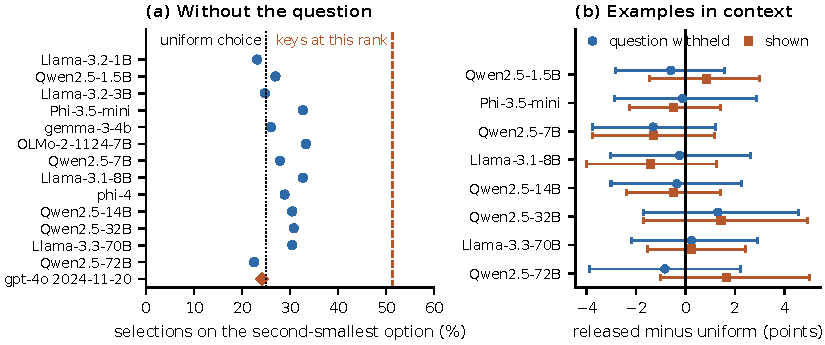
\includegraphics[width=\linewidth]{figures/norank.pdf}
\caption{\textbf{No model we tested picks v1.5's second-smallest option as often as the key sits there.} \textbf{(a)} The share of each model's selections that fall on the second-smallest of v1.5's four numeric options,
with the question withheld, against the share of keys there and the share a uniform choice gives. Each model answers
BixBench's template once per prompt, in three letter orderings of each of the $105$ items, and we take the letter it
rates most likely \citep{multiplechoiceability}. \textbf{(b)} Solved v1.5 items from other capsules shown as examples:
accuracy with $64$ examples whose keys sit at their released ranks minus accuracy with the same examples redrawn to a
uniform rank, with the question withheld and shown. Plain $95\%$ intervals over $46$ capsules; eight draws of examples
and orderings per item.}
\label{fig:norank}
\end{figure}

\begin{figure}[htbp]
\centering\footnotesize
\fbox{\begin{minipage}{0.95\linewidth}\raggedright\sloppy
\textbf{The two prompts for choosing among the options without the data}, verbatim, with the prompts' own line
breaks shown as line breaks, here with the question withheld. Figure~\ref{fig:norank} uses the template;
Table~\ref{tab:gptnodata} uses both.

\smallskip
\emph{Template.} BixBench's own, verbatim; the missing line break before \textsc{important} is in the
original:

{\ttfamily\scriptsize Extract the single letter answer to the following question from the given
options. You must pick one answer even if you are unsure.\par\smallskip
Question: \{question\}\par\smallskip
Options:\par
\{options\}IMPORTANT: You must only output a single letter answer in XML format.\par\smallskip
\ Example Output: <answer> X </answer>\par}

\smallskip
\emph{Chat prompt.} System message, then user message. Its instruction does not refer to the options:

{\ttfamily\scriptsize You are answering a multiple-choice question. Think it through, then reply
with a single final line in exactly this form:\par
FINAL: <letter>\par\smallskip
Question: [withheld]\par\smallskip
Options:\par
(A) \ldots\par}

\end{minipage}}
\caption{The prompts for choosing without the data.}
\label{fig:prompts}
\end{figure}

\FloatBarrier
\subsection{The cost of hiding the rank}
\label{app:replication}

\paragraph{With the data.} Among the agents that call tools in text, one uses the data: Qwen2.5-72B's submitted number
is within $5\%$ of the key on $14.3\%$ of the numeric items, against $1.0\%$ without the data. Yet no grading through
options shows its lead over the other two in-text agents with an interval that excludes zero
(Figure~\ref{fig:withdata}b). Table~\ref{tab:withdata} scores each configuration with and without the data,
Figure~\ref{fig:withdata}a grades the same runs through $R$, $P$ and $U$, and Table~\ref{tab:mechanism} counts what $U$
newly accepts on the moved keys.

\begin{figure}[htbp]
\centering
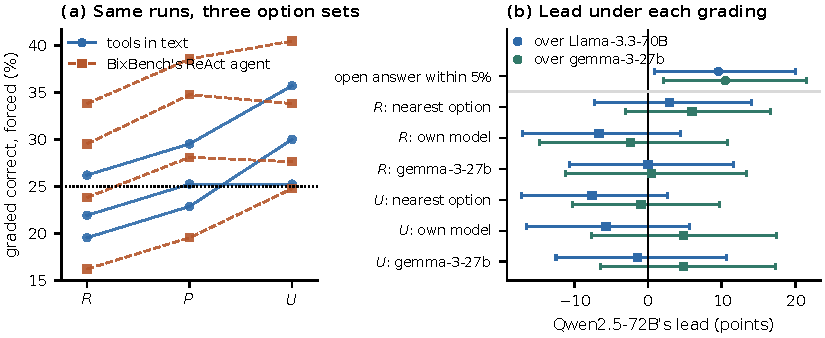
\includegraphics[width=\linewidth]{figures/withdata.pdf}
\caption{\textbf{The same runs, graded through different options.} \textbf{(a)} The seven configurations' runs with the
data, graded forced by each configuration's own model (Qwen3-30B-A3B's runs by gemma-3-27b) on the $105$ numeric items
through $R$, $P$ and $U$. The dotted line is chance. \textbf{(b)} Qwen2.5-72B's lead with the data over the other two
in-text agents, by the share of answers within $5\%$ of the key and by three gradings of the same runs through $R$ and
$U$: the nearest-option rule, each configuration's own model and gemma-3-27b. Intervals paired over $46$ capsules at $96\%$.}
\label{fig:withdata}
\end{figure}

\begin{table}[htbp]
\centering\footnotesize\setlength{\tabcolsep}{2.3pt}
\caption{BixBench's agent with and without each capsule's data: three open-weight models writing tool calls as
text, and four running BixBench's ReAct agent. Each configuration is graded by its own model, as the published runs
were, except $^\dagger$Qwen3-30B-A3B, graded by gemma-3-27b because its own grading, with replies cut at $1{,}536$
tokens before the answer, selects no option on $51.7$ and $63.3\%$ of its forced gradings through $R$ with and without
the data (its open-ended grades are its own). \emph{Open}: BixBench v1.5's
graders on all $205$ items; \emph{within $5\%$}: the submitted number within $5\%$ of the key on the $105$ numeric items, as the tolerance reads it. \emph{Multiple choice}: BixBench's multiple-choice grader on all $205$ with the
released options, forced and with BixBench's ``insufficient information'' option; in parentheses, the share of graded
runs (those with an answer) that select that option. The last four columns grade the \emph{same} runs on the $105$ numeric
items through the three
option sets, so a difference between them is due to the option set alone; $R-U$'s interval is paired over $46$
capsules at $96.0\%$, the level that attains $95\%$ coverage. Chance is $25\%$ forced and $20\%$ when the
grader may refuse.}
\label{tab:withdata}
\begin{tabular}{llrrrrrrrr}
\toprule
& & \multicolumn{2}{c}{open answer} & \multicolumn{2}{c}{multiple choice, all $205$} &
\multicolumn{4}{c}{the same runs, $105$ numeric items, forced}\\
\cmidrule(lr){3-4}\cmidrule(lr){5-6}\cmidrule(lr){7-10}
Agent & data & graders & within $5\%$ & forced & with refusal & $R$ & $P$ & $U$ & $R-U$\\
\midrule
\multicolumn{10}{l}{\emph{tools called in text}}\\
Qwen2.5-72B & with & $18.0$ & $14.3$ & $27.6$ & $20.0$ $(47)$ & $19.5$ & $22.9$ & $30.0$ & $-10.5$ $[-16.3,-5.2]$\\
 & without & $6.8$ & $1.0$ & $17.8$ & $8.0$ $(67)$ & $16.7$ & $18.1$ & $25.7$ & $-9.0$ $[-17.6,-1.0]$\\
Llama-3.3-70B & with & $6.3$ & $4.8$ & $25.9$ & $8.0$ $(70)$ & $26.2$ & $29.5$ & $35.7$ & $-9.5$ $[-15.7,-3.1]$\\
 & without & $9.8$ & $4.8$ & $27.1$ & $11.0$ $(72)$ & $24.8$ & $30.0$ & $31.9$ & $-7.1$ $[-15.0,-0.4]$\\
gemma-3-27b & with & $4.4$ & $3.8$ & $21.7$ & $9.0$ $(62)$ & $21.9$ & $25.2$ & $25.2$ & $-3.3$ $[-7.1,+0.0]$\\
 & without & $5.9$ & $3.8$ & $23.4$ & $8.3$ $(60)$ & $22.4$ & $24.3$ & $25.2$ & $-2.9$ $[-8.5,+2.5]$\\
\midrule
\multicolumn{10}{l}{\emph{BixBench's ReAct agent, tools passed through the server's interface}}\\
Qwen2.5-72B & with & $10.7$ & $9.5$ & $19.3$ & $12.4$ $(56)$ & $16.2$ & $19.5$ & $24.8$ & $-8.6$ $[-15.1,-1.8]$\\
 & without & $5.4$ & $2.9$ & $19.5$ & $6.8$ $(73)$ & $17.1$ & $17.1$ & $17.1$ & $+0.0$ $[-6.5,+6.1]$\\
Llama-3.3-70B & with & $9.8$ & $5.7$ & $30.5$ & $6.6$ $(87)$ & $29.5$ & $34.8$ & $33.8$ & $-4.3$ $[-10.9,+1.8]$\\
 & without & $4.9$ & $1.9$ & $22.0$ & $0.5$ $(94)$ & $21.4$ & $22.4$ & $26.7$ & $-5.2$ $[-10.3,-0.4]$\\
GLM-4.5-Air & with & $27.3$ & $16.2$ & $42.9$ & $28.3$ $(55)$ & $33.8$ & $38.6$ & $40.5$ & $-6.7$ $[-13.9,+0.6]$\\
 & without & $6.3$ & $4.8$ & $24.1$ & $11.2$ $(63)$ & $24.8$ & $26.7$ & $30.0$ & $-5.2$ $[-10.9,+0.9]$\\
Qwen3-30B-A3B$^\dagger$ & with & $18.0$ & $14.3$ & $32.7$ & $21.7$ $(50)$ & $23.8$ & $28.1$ & $27.6$ & $-3.8$ $[-8.2,+0.0]$\\
 & without & $3.4$ & $1.9$ & $14.9$ & $7.8$ $(61)$ & $13.3$ & $17.1$ & $17.6$ & $-4.3$ $[-9.5,+0.5]$\\
\bottomrule
\end{tabular}
\end{table}

\begin{table}[htbp]
\centering\footnotesize\setlength{\tabcolsep}{2.6pt}
\caption{What $U$ accepts on the $37$ moved keys, per configuration. \emph{Newly accepted}: answers that the
nearest-option rule grades correct under $U$ but not under $R$, by the submitted number's relative distance from the
key; \emph{open side}: those of them on the key's open side. \emph{Without the data}: the same count for the agents'
runs without the data. \emph{$U-P$}: on the moved keys, with an interval over their $21$ capsules at
$97.75\%$, the level that attains $95\%$ coverage there, and on the $12$ inward and $56$ unchanged keys.}
\label{tab:mechanism}
\begin{tabular}{lrrrrrrrrr}
\toprule
& \multicolumn{5}{c}{newly accepted, with the data} & without & \multicolumn{3}{c}{$U-P$}\\
\cmidrule(lr){2-6}\cmidrule(lr){7-7}\cmidrule(lr){8-10}
agent & ${\le}5\%$ & $5$--$25\%$ & $25$--$100\%$ & ${>}100\%$ & open side & the data & moved & inward & unchanged\\
\midrule
\multicolumn{10}{l}{\emph{tools called in text}}\\
Qwen2.5-72B & $1$ & $0$ & $2$ & $1$ & $4$ & $5$ & $+13.5$ $[+0.0,+28.9]$ & $-8.3$ & $+0.0$\\
Llama-3.3-70B & $0$ & $2$ & $9$ & $2$ & $13$ & $12$ & $+27.0$ $[+9.7,+45.5]$ & $-8.3$ & $+1.8$\\
gemma-3-27b & $0$ & $0$ & $4$ & $4$ & $8$ & $9$ & $+18.2$ $[+4.4,+34.6]$ & $+0.0$ & $+1.8$\\
\addlinespace
\multicolumn{10}{l}{\emph{BixBench's ReAct agent}}\\
Qwen2.5-72B & $1$ & $0$ & $2$ & $2$ & $5$ & $4$ & $+12.8$ $[+0.0,+26.3]$ & $-8.3$ & $+0.0$\\
Llama-3.3-70B & $0$ & $1$ & $4$ & $3$ & $8$ & $6$ & $+21.6$ $[+5.7,+38.9]$ & $-8.3$ & $+3.6$\\
GLM-4.5-Air & $0$ & $1$ & $2$ & $1$ & $3$ & $7$ & $+10.1$ $[+0.0,+23.0]$ & $-16.7$ & $+0.0$\\
Qwen3-30B-A3B$^\dagger$ & $1$ & $0$ & $1$ & $3$ & $5$ & $4$ & $+13.5$ $[+2.6,+28.2]$ & $-16.7$ & $+0.0$\\
\bottomrule
\end{tabular}
\end{table}

\paragraph{The pre-specified test.} We fixed the data, the option sets, the key groups, the grading rule, the
statistics and a pass criterion for each hypothesis (Table~\ref{tab:predictions}) in a plan dated 24 September 2026,
before the published runs were analysed and before the new runs were made. We committed the plan to our version history and
pushed it to GitHub, whose push record, archived with the code, dates the push at 16:25 UTC, $15$ minutes before the
push of the first results. The new runs, $3{,}280$ question runs with and without the data, are two runs of Qwen3-235B-A22B and
two new seeds of each in-text agent on all $205$ questions. On the published runs, $U$ moves $11$ unchanged keys
from one extreme to the other, which changes their open side (\S\ref{sec:cost}); on them $U-R$ is $+19.1$ points. For
Qwen3-235B-A22B, the redrawing itself accepts near misses: on its unchanged keys whose rank $U$ leaves as released, $U$ gains
$+6.7$ points against $R$ and $+1.7$ against $P$.

\begin{table}[htbp]
\centering\scriptsize\setlength{\tabcolsep}{2.5pt}
\caption{\textbf{The hypotheses of the pre-specified test and their results.} Each hypothesis, its pass
criterion (abbreviated) and each run set's estimate: the nearest-option rule's $U-R$ in points unless stated otherwise,
with the data (H6: without it), and the interval fixed in advance. H3: the shares of newly accepted answers more than
$25\%$ from the key and on its open side. \emph{pass} or \textbf{fail} is the verdict
under the stated criterion, except where marked. $^{\ddagger}$No interval reaches $95\%$ coverage on these
$12$ keys in $10$ capsules; H5's criterion uses the mean alone, so this pass carries no uncertainty statement.
$^{\S}$The stated criterion passes it only by its $5$-point clause; the interval excludes $0$, so we count it
as failed. We added the last row, H2 as an equivalence claim (the whole interval within $\pm5$ points of zero, ruling out a
change larger than $5$ points), after the results; it is not part of the plan.}
\label{tab:predictions}
\begin{tabularx}{\linewidth}{@{}p{2.2cm}Xp{2.35cm}p{2.35cm}p{2.35cm}@{}}
\toprule
hypothesis & pass criterion & v1.0: gpt-4o, Claude 3.5 & v1.5: new seeds & v1.5: Qwen3-235B-A22B\\
\midrule
H1: moved keys gain & the interval's lower end is above 0 & $+19.8$ {\scriptsize$[+10.4,+31.2]$} pass & $+17.6$ {\scriptsize$[+9.0,+25.8]$} pass & $+9.5$ {\scriptsize$[+0.0,+22.1]$} \textbf{fail}\\
H2: unchanged keys do not & an interval that contains 0, or a mean within 5 points of 0 & $+3.7$ {\scriptsize$[+0.9,+6.9]$} \textbf{fail}$^{\S}$ & $+2.9$ {\scriptsize$[-0.2,+7.0]$} pass & $+8.9$ {\scriptsize$[+2.7,+16.3]$} \textbf{fail}\\
H3: newly accepted answers are far and on the open side & more than half are more than 25\% from the key, and more than half lie beyond the key on the side without a distractor & $91$, $96\%$ of $283$ pass & $93$, $98\%$ of $42$ pass & $86$, $100\%$ of $7$ pass\\
H4: not the redrawing & $U-P$ on moved keys: the interval's lower end is above 0 & $+18.6$ {\scriptsize$[+8.7,+30.7]$} pass & $+17.9$ {\scriptsize$[+9.9,+25.5]$} pass & $+4.7$ {\scriptsize$[-0.8,+9.7]$} \textbf{fail}\\
H5: inward keys do not gain & a mean of at most 0 & $-14.2$ {\scriptsize$[-20.6,-8.2]$} pass & $-8.3$ {\scriptsize$[-22.2,+0.0]$} pass & $-12.5$$^{\ddagger}$ pass\\
H6: the gain needs no data & without the data, the moved keys' interval's lower end is above 0 & -- & $+22.2$ {\scriptsize$[+14.2,+30.9]$} pass & $+21.6$ {\scriptsize$[+10.0,+33.8]$} pass\\
H2 as equivalence & the whole interval within $\pm5$ points & not shown (upper end $+6.9$) & not shown (upper end $+7.0$) & not shown (upper end $+16.3$)\\
\bottomrule
\end{tabularx}
\end{table}

\begin{table}[htbp]
\centering\scriptsize\setlength{\tabcolsep}{3pt}
\caption{\textbf{The pre-specified test with the number read as the tolerance reads it.} Each hypothesis of
Table~\ref{tab:predictions} on each run set, with the nearest-option rule reading the last number in the answer
rather than reading a number only when the whole answer is one. The statistics, levels and criteria are the same, with
H2 counted as failed wherever its interval excludes zero; the whole-answer reading reproduces
Table~\ref{tab:predictions} exactly.
$^{\ddagger}$No interval reaches $95\%$ coverage on these keys.}
\label{tab:lastnumber}
\begin{tabular}{llll}
\toprule
hypothesis & v1.0: gpt-4o, Claude 3.5 & v1.5: new seeds & v1.5: Qwen3-235B-A22B\\
\midrule
H1: moved keys gain & $+23.2$ {\scriptsize$[+13.3,+34.8]$} pass & $+23.0$ {\scriptsize$[+12.3,+32.9]$} pass & $+9.5$ {\scriptsize$[+0.0,+22.1]$} \textbf{fail}\\
H2: unchanged keys do not & $+4.7$ {\scriptsize$[+1.9,+8.0]$} \textbf{fail} & $+2.9$ {\scriptsize$[-1.2,+9.3]$} pass & $+8.9$ {\scriptsize$[+2.7,+16.3]$} \textbf{fail}\\
H3: far, on the open side & $92$, $96\%$ of $329$ pass & $95$, $98\%$ of $55$ pass & $86$, $100\%$ of $7$ pass\\
H4: not the redrawing & $+21.9$ {\scriptsize$[+11.2,+35.1]$} pass & $+24.2$ {\scriptsize$[+13.8,+33.8]$} pass & $+4.7$ {\scriptsize$[-0.8,+9.7]$} \textbf{fail}\\
H5: inward keys do not gain & $-13.9$ {\scriptsize$[-20.5,-7.9]$} pass & $-11.1$$^{\ddagger}$ pass & $-12.5$$^{\ddagger}$ pass\\
H6: the gain needs no data & -- & $+32.5$ {\scriptsize$[+20.0,+45.2]$} pass & $+21.6$ {\scriptsize$[+10.0,+33.8]$} pass\\
\bottomrule
\end{tabular}
\end{table}

\paragraph{Other graders.} Tables~\ref{tab:readers2}, \ref{tab:readersfull} and~\ref{tab:variants} give every
grading's differences. With BixBench's prompt and the notebook, Qwen2.5-72B and Llama-3.3-70B graded a random quarter
of the published runs and every run on a moved key, and gemma-3-27b graded every run of the test. To measure
$\lambda$, we take the option nearest the number the tolerance reads (ties in $d$ broken by $|a-v|$) and pool every
option set. The proximity weight predicts which graders bear more of the rule's cost, but the size of that cost only roughly. Over the $46$ gradings of Figure~\ref{fig:cost}a, a
grading's share of the rule's cost rises with its $\lambda$ (rank correlation $0.88$), but the cost $\lambda$ predicts
falls short of the answer-only graders' on the published runs and exceeds the notebook graders' on the new seeds.
Estimated from the unchanged and inward keys alone, $\lambda$ predicts the moved keys' cost with an error of $3.9$ points
on average over the $42$ gradings that also graded those keys, and the observed cost lies within its prediction's
interval for $18$ of the $42$; Table~\ref{tab:variants}'s \emph{predicted} column uses $\lambda$ from all keys. On the moved keys the answer-only graders bear $74$ to $90\%$ of the nearest-option rule's cost on the
same answers, the rule reading the number as the tolerance does. With the within-$5\%$ option they select that option on $80.1$ to $91.5\%$ of the
published runs' misses and on $5.8$ to $12.3\%$ of their correct answers; counting wrong selections too, they reject
$6.6$ to $17.9\%$ of the correct answers on the two releases.

\begin{table}[htbp]
\centering\footnotesize\setlength{\tabcolsep}{3pt}
\caption{\textbf{Graders bear the cost of hiding the rank in the order of their proximity weight.} $U-P$ in
points on the moved keys ($41$ on v1.0, $40$ of them also redrawn by $P$; $37$ on v1.5), with its interval and
the sign-flip test's $p$-value, and over all numeric items. $\lambda$: the grading's proximity weight
(Remark~\ref{rem:lambda}), from its own selections on the misses of the same runs. \emph{Nearest
option}: the rule of the pre-specified test, the only row fixed before its data were analysed;
\emph{published}: BixBench's own forced grades, which exist only for $R$ ($\lambda$ pooled over both models:
$0.24$ for gpt-4o's grades, $0.58$ for Claude 3.5 Sonnet's); \emph{answer-only}, \emph{letter only}, \emph{refusal} and
\emph{within $5\%$}: as in Table~\ref{tab:glossary}. The other graders read the notebook under
BixBench's prompt; gpt-4o is version 2024-11-20. On the new seeds, Qwen2.5-72B and Llama-3.3-70B graded only
the moved keys. Double-bootstrap intervals over each group's capsules ($^{\ddagger}$no level attains $95\%$
coverage); every difference is in Tables~\ref{tab:readersfull} and~\ref{tab:variants}.}
\label{tab:readers2}
\begin{tabular}{llrrrr}
\toprule
& & & \multicolumn{2}{c}{moved keys} & all\\
\cmidrule(lr){4-5}
runs & grader & $\lambda$ & $U-P$ & $p$ & $U-P$\\
\midrule
v1.0, published & nearest option & $1$ & $+18.6$ {\scriptsize$[+8.7,+30.7]$} & $<0.001$ & $+3.4$\\
 & published & $0.44$ & -- & -- & --\\
 & gpt-4o, answer-only & $0.69$ & $+27.2$ {\scriptsize$[+14.7,+38.5]$} & $<0.001$ & $+4.0$\\
 & gemma-3-27b, answer-only & $0.62$ & $+28.2$ {\scriptsize$[+17.4,+39.4]$} & $<0.001$ & $+3.9$\\
 & Qwen2.5-72B & $0.43$ & $+14.4$ {\scriptsize$[+7.0,+22.2]$} & $<0.001$ & $+0.5$\\
 & gemma-3-27b & $0.29$ & $+8.7$ {\scriptsize$[+4.3,+14.0]$} & $<0.001$ & $+0.7$\\
 & gpt-4o, letter only & $0.24$ & $+6.6$ {\scriptsize$[+2.0,+12.1]$} & $<0.001$ & $+0.4$\\
 & Llama-3.3-70B & $0.22$ & $+8.8$ {\scriptsize$[+3.7,+14.1]$} & $<0.001$ & $+3.0$\\
 & gemma-3-27b, refusal & $0.18$ & $+3.2$ {\scriptsize$[+0.4,+7.3]$} & $0.003$ & $+0.5$\\
 & gpt-4o & $0.17$ & $+5.9$ {\scriptsize$[+1.0,+11.2]$} & $0.014$ & $+0.7$\\
 & gemma-3-27b, within $5\%$ & $0.08$ & $-0.1$ {\scriptsize$[-0.7,+0.3]$} & $0.500$ & $+0.1$\\
v1.5, new seeds & nearest option & $1$ & $+17.9$ {\scriptsize$[+9.9,+25.5]$} & $<0.001$ & $+6.6$\\
 & gpt-4o, answer-only & $0.65$ & $+21.2$ {\scriptsize$[+11.9,+30.6]$} & $<0.001$ & $+5.0$\\
 & gemma-3-27b, answer-only & $0.60$ & $+21.8$ {\scriptsize$[+15.1,+28.8]$} & $<0.001$ & $+6.6$\\
 & Qwen2.5-72B & $0.40$ & $+6.8$ {\scriptsize$[+0.2,+13.6]$} & $0.059$ & --\\
 & gemma-3-27b & $0.20$ & $+0.7$ {\scriptsize$[-4.8,+5.7]$} & $0.861$ & $+0.5$\\
 & Llama-3.3-70B & $0.18$ & $+4.5$ {\scriptsize$[-2.5,+11.1]$} & $0.178$ & --\\
 & gemma-3-27b, refusal & $0.12$ & $+2.5$ {\scriptsize$[-0.2,+5.8]$} & $0.055$ & $+1.2$\\
 & gemma-3-27b, within $5\%$ & $0.06$ & $-0.2$$^{\ddagger}$ & $1.000$ & $-0.2$\\
\bottomrule
\end{tabular}
\end{table}

\begin{table}[htbp]
\centering\scriptsize\setlength{\tabcolsep}{1.8pt}
\caption{\textbf{All gradings of the same runs, all differences.} Differences between gradings of the same
with-data runs through two option sets, in points. On the moved keys ($37$ on v1.5; $41$ on v1.0, $40$ of
them also redrawn by $P$): $U-P$ (the rank alone), $P-R$ (the redrawing alone) and $U-R$; on the unchanged keys
and over all numeric items, $U-P$. Graders as in Table~\ref{tab:readers2}; on the v1.5 runs, Qwen2.5-72B and
Llama-3.3-70B graded only the moved keys (--: not graded). Configurations pooled as in the pre-specified test; no row of this table is part of it.
Intervals as in Appendix~\ref{app:stats} ($^{\ddagger}$no level attains $95\%$ coverage); $p$: the sign-flip test of $U-P$ on the moved keys.}
\label{tab:readersfull}
\resizebox{\linewidth}{!}{\begin{tabular}{llrrrrrr}
\toprule
& & \multicolumn{3}{c}{moved keys} & unchanged & all & \\
\cmidrule(lr){3-5}\cmidrule(lr){6-6}\cmidrule(lr){7-7}
runs & grader & $U-P$ & $P-R$ & $U-R$ & $U-P$ & $U-P$ & $p$\\
\midrule
v1.5, seven configurations & nearest option & $+16.7$ & $+1.1$ & $+17.8$ & $+1.0$ & $+5.3$ & $<0.001$\\
 & & {\scriptsize$[+10.2,+23.0]$} & {\scriptsize$[-2.0,+4.4]$} & {\scriptsize$[+11.3,+24.9]$} & {\scriptsize$\ddagger$} & {\scriptsize$[+1.9,+8.6]$} & \\
 & own model & $+5.8$ & $+6.4$ & $+12.2$ & $+1.4$ & $+2.7$ & $0.037$\\
 & & {\scriptsize$[+1.2,+10.4]$} & {\scriptsize$[+2.7,+10.2]$} & {\scriptsize$[+6.2,+18.1]$} & {\scriptsize$[-1.7,+4.3]$} & {\scriptsize$[+0.2,+5.3]$} & \\
 & gemma-3-27b & $+4.6$ & $+3.5$ & $+8.1$ & $+1.8$ & $+2.6$ & $0.108$\\
 & & {\scriptsize$[-0.9,+9.8]$} & {\scriptsize$[-0.7,+9.9]$} & {\scriptsize$[+3.7,+13.2]$} & {\scriptsize$[-1.1,+4.8]$} & {\scriptsize$[+0.1,+5.1]$} & \\
 & gemma-3-27b, refusal & $+1.4$ & $+1.0$ & $+2.3$ & $+1.0$ & $+1.0$ & $0.312$\\
 & & {\scriptsize$[-0.9,+3.8]$} & {\scriptsize$[-1.4,+3.0]$} & {\scriptsize$[-0.4,+5.6]$} & {\scriptsize$[-0.4,+2.6]$} & {\scriptsize$[-0.1,+2.0]$} & \\
 & Qwen2.5-72B & $+10.2$ & $+3.5$ & $+13.7$ & -- & -- & $0.001$\\
 & & {\scriptsize$[+4.5,+15.9]$} & {\scriptsize$[-1.8,+8.0]$} & {\scriptsize$[+6.1,+20.5]$} &  &  & \\
 & Llama-3.3-70B & $+0.4$ & $+6.0$ & $+6.4$ & -- & -- & $0.928$\\
 & & {\scriptsize$[-4.4,+5.0]$} & {\scriptsize$[+2.9,+9.4]$} & {\scriptsize$[+0.2,+12.4]$} &  &  & \\
v1.0, published & gpt-4o & $+5.9$ & $+0.3$ & $+6.1$ & $+1.4$ & $+0.7$ & $0.014$\\
 & & {\scriptsize$[+1.0,+11.2]$} & {\scriptsize$[-1.6,+2.4]$} & {\scriptsize$[+1.5,+11.3]$} & {\scriptsize$[-1.7,+4.4]$} & {\scriptsize$[-2.4,+3.9]$} & \\
 & gemma-3-27b & $+8.7$ & $+1.3$ & $+9.8$ & $+1.0$ & $+0.7$ & $<0.001$\\
 & & {\scriptsize$[+4.3,+14.0]$} & {\scriptsize$[-0.8,+3.5]$} & {\scriptsize$[+5.1,+15.4]$} & {\scriptsize$[-0.8,+3.1]$} & {\scriptsize$[-2.2,+3.3]$} & \\
 & gemma-3-27b, refusal & $+3.2$ & $+0.1$ & $+3.2$ & $+0.2$ & $+0.5$ & $0.003$\\
 & & {\scriptsize$[+0.4,+7.3]$} & {\scriptsize$[-1.3,+1.4]$} & {\scriptsize$[+0.8,+6.6]$} & {\scriptsize$[-1.9,+2.2]$} & {\scriptsize$[-0.7,+1.8]$} & \\
 & Qwen2.5-72B & $+14.4$ & $+1.3$ & $+15.4$ & $+0.8$ & $+0.5$ & $<0.001$\\
 & & {\scriptsize$[+7.0,+22.2]$} & {\scriptsize$[-1.1,+3.7]$} & {\scriptsize$[+7.9,+23.3]$} & {\scriptsize$[-3.7,+5.9]$} & {\scriptsize$[-3.5,+4.7]$} & \\
 & Llama-3.3-70B & $+8.8$ & $-1.5$ & $+7.1$ & $+3.7$ & $+3.0$ & $<0.001$\\
 & & {\scriptsize$[+3.7,+14.1]$} & {\scriptsize$[-4.9,+1.5]$} & {\scriptsize$[+1.5,+13.1]$} & {\scriptsize$[+0.3,+7.3]$} & {\scriptsize$[+0.1,+6.0]$} & \\
v1.5, new seeds & gemma-3-27b & $+0.7$ & $+3.6$ & $+4.3$ & $+1.5$ & $+0.5$ & $0.861$\\
 & & {\scriptsize$[-4.8,+5.7]$} & {\scriptsize$[-0.2,+7.9]$} & {\scriptsize$[-0.7,+9.3]$} & {\scriptsize$[-2.9,+5.0]$} & {\scriptsize$[-2.4,+3.3]$} & \\
 & gemma-3-27b, refusal & $+2.5$ & $+0.0$ & $+2.5$ & $+0.6$ & $+1.2$ & $0.055$\\
 & & {\scriptsize$[-0.2,+5.8]$} & {\scriptsize$[-2.7,+2.7]$} & {\scriptsize$[-1.2,+7.1]$} & {\scriptsize$[-1.0,+2.5]$} & {\scriptsize$[-0.1,+2.7]$} & \\
 & Qwen2.5-72B & $+6.8$ & $+4.1$ & $+10.8$ & -- & -- & $0.059$\\
 & & {\scriptsize$[+0.2,+13.6]$} & {\scriptsize$[-3.2,+11.1]$} & {\scriptsize$[+4.0,+17.5]$} &  &  & \\
 & Llama-3.3-70B & $+4.5$ & $+2.5$ & $+7.0$ & -- & -- & $0.178$\\
 & & {\scriptsize$[-2.5,+11.1]$} & {\scriptsize$[-1.2,+5.8]$} & {\scriptsize$[-1.3,+14.5]$} &  &  & \\
v1.5, Qwen3-235B-A22B & gemma-3-27b & $+1.4$ & $+4.1$ & $+5.4$ & $-2.7$ & $-1.2$ & $0.797$\\
 & & {\scriptsize$[-4.6,+6.7]$} & {\scriptsize$[+0.6,+9.7]$} & {\scriptsize$[-0.7,+12.5]$} & {\scriptsize$[-7.0,+1.0]$} & {\scriptsize$[-3.8,+1.2]$} & \\
 & gemma-3-27b, refusal & $+0.7$ & $+3.4$ & $+4.1$ & $+0.4$ & $+0.5$ & $1.000$\\
 & & {\scriptsize$\ddagger$} & {\scriptsize$[-1.5,+10.5]$} & {\scriptsize$[+0.7,+8.3]$} & {\scriptsize$[-3.0,+3.7]$} & {\scriptsize$[-1.4,+2.5]$} & \\
 & Qwen2.5-72B & $+2.7$ & $+4.1$ & $+6.8$ & -- & -- & $0.591$\\
 & & {\scriptsize$[-5.3,+10.8]$} & {\scriptsize$[-3.4,+13.5]$} & {\scriptsize$[-1.8,+15.8]$} &  &  & \\
 & Llama-3.3-70B & $+4.7$ & $+0.7$ & $+5.4$ & -- & -- & $0.243$\\
 & & {\scriptsize$[-2.2,+12.5]$} & {\scriptsize$[-4.5,+5.4]$} & {\scriptsize$[-3.5,+15.4]$} &  &  & \\
\bottomrule
\end{tabular}}
\end{table}

\begin{table}[htbp]
\centering\scriptsize\setlength{\tabcolsep}{1.6pt}
\caption{\textbf{The rank's cost under the other gradings.} The same with-data runs as
Table~\ref{tab:readers2}. $\lambda$: the proximity weight; $U-P$ on the moved keys with the sign-flip test's
$p$, through the original rewrites and through the digit-matched $P'$ and $U'$ (which move $42$ keys on v1.0 and
$36$ on v1.5); $U-P$ on the unchanged keys and over all numeric items; and the cost on the moved keys that
$\lambda$ predicts (Remark~\ref{rem:lambda}). Graders as in Table~\ref{tab:readers2}; rows without a suffix:
BixBench's prompt with the notebook, graded here through $P'$ and $U'$ only (their $U-P$ is in Table~\ref{tab:readersfull}).
Intervals as in Table~\ref{tab:readers2} ($^{\ddagger}$no level attains $95\%$ coverage); no row is part of the
pre-specified test.}
\label{tab:variants}
\resizebox{\linewidth}{!}{\begin{tabular}{lrrrrrrrr}
\toprule
& & \multicolumn{2}{c}{$U-P$, moved} & \multicolumn{2}{c}{$U'-P'$, moved} & unchanged & all & \\
\cmidrule(lr){3-4}\cmidrule(lr){5-6}
grader & $\lambda$ & & $p$ & & $p$ & $U-P$ & $U-P$ & predicted\\
\midrule
\multicolumn{9}{l}{\emph{BixBench's published runs (v1.0)}}\\
gpt-4o, answer-only & $0.69$ & $+27.2$ {\scriptsize$[+14.7,+38.5]$} & $<0.001$ & $+29.7$ {\scriptsize$[+18.0,+41.1]$} & $<0.001$ & $+4.1$ & $+4.0$ & $+22.1$\\
gemma-3-27b, answer-only & $0.62$ & $+28.2$ {\scriptsize$[+17.4,+39.4]$} & $<0.001$ & $+28.2$ {\scriptsize$[+18.5,+38.0]$} & $<0.001$ & $+2.0$ & $+3.9$ & $+20.0$\\
Qwen2.5-72B, answer-only & $0.58$ & $+24.7$ {\scriptsize$[+6.3,+42.9]$} & $0.004$ & $+28.8$ {\scriptsize$[+14.8,+42.3]$} & $<0.001$ & $+2.5$ & $+2.1$ & $+18.6$\\
Llama-3.3-70B, answer-only & $0.48$ & $+23.4$ {\scriptsize$[+11.9,+34.9]$} & $<0.001$ & $+19.7$ {\scriptsize$[+7.7,+31.9]$} & $0.002$ & $+3.3$ & $+3.5$ & $+15.5$\\
Qwen2.5-72B & $0.43$ & -- & -- & $+14.0$ {\scriptsize$[+4.7,+24.9]$} & $<0.001$ & -- & -- & $+12.5$\\
gemma-3-27b & $0.27$ & -- & -- & $+7.3$ {\scriptsize$[+2.4,+12.2]$} & $0.003$ & -- & -- & $+7.8$\\
gpt-4o, letter only & $0.24$ & $+6.6$ {\scriptsize$[+2.0,+12.1]$} & $<0.001$ & $+5.3$ {\scriptsize$[-0.3,+11.0]$} & $0.061$ & $+0.5$ & $+0.4$ & $+7.6$\\
Llama-3.3-70B & $0.21$ & -- & -- & $+5.6$ {\scriptsize$[+0.0,+11.2]$} & $0.048$ & -- & -- & $+6.1$\\
gemma-3-27b, within $5\%$ & $0.08$ & $-0.1$ {\scriptsize$[-0.7,+0.3]$} & $0.500$ & $-0.8$ {\scriptsize$[-1.7,-0.1]$} & $0.016$ & $+0.2$ & $+0.1$ & $+2.5$\\
gpt-4o, within $5\%$ & $0.08$ & $-1.1$$^{\ddagger}$ & $0.548$ & $-1.7$$^{\ddagger}$ & $0.321$ & $+0.5$ & $+0.1$ & $+2.5$\\
Qwen2.5-72B, within $5\%$ & $0.06$ & $-1.1$$^{\ddagger}$ & $0.267$ & $-1.3$$^{\ddagger}$ & $0.142$ & $+0.1$ & $-0.0$ & $+1.9$\\
\multicolumn{9}{l}{\emph{our seven configurations (v1.5)}}\\
gpt-4o, answer-only & $0.60$ & $+18.5$ {\scriptsize$[+11.7,+24.9]$} & $<0.001$ & $+19.9$ {\scriptsize$[+12.1,+29.1]$} & $<0.001$ & $-2.0$ & $+4.3$ & $+20.7$\\
gemma-3-27b, answer-only & $0.54$ & $+22.0$ {\scriptsize$[+14.9,+29.0]$} & $<0.001$ & $+21.6$ {\scriptsize$[+13.7,+30.0]$} & $<0.001$ & $+1.7$ & $+7.3$ & $+18.9$\\
Qwen2.5-72B, answer-only & $0.49$ & $+21.6$ {\scriptsize$[+13.5,+29.0]$} & $<0.001$ & $+21.2$ {\scriptsize$[+13.8,+29.5]$} & $<0.001$ & $+1.7$ & $+7.3$ & $+17.0$\\
Llama-3.3-70B, answer-only & $0.42$ & $+15.3$ {\scriptsize$[+7.1,+23.4]$} & $0.002$ & $+11.0$ {\scriptsize$[+1.1,+21.7]$} & $0.041$ & $+1.4$ & $+5.1$ & $+14.8$\\
Qwen2.5-72B & $0.36$ & -- & -- & $+12.8$ {\scriptsize$[+6.9,+19.0]$} & $<0.001$ & -- & -- & $+12.4$\\
gemma-3-27b & $0.24$ & -- & -- & $+5.8$ {\scriptsize$[+2.3,+9.4]$} & $0.011$ & -- & -- & $+8.4$\\
Llama-3.3-70B & $0.22$ & -- & -- & $+2.6$ {\scriptsize$[-0.7,+6.0]$} & $0.114$ & -- & -- & $+7.5$\\
gemma-3-27b, within $5\%$ & $0.07$ & $-0.2$$^{\ddagger}$ & $1.000$ & $-0.2$$^{\ddagger}$ & $1.000$ & $+0.1$ & $+0.0$ & $+2.5$\\
gpt-4o, within $5\%$ & $0.06$ & $-1.4$ {\scriptsize$[-3.2,+0.4]$} & $0.249$ & $-3.9$ {\scriptsize$[-9.8,+0.0]$} & $0.125$ & $-0.4$ & $-0.7$ & $+2.2$\\
Qwen2.5-72B, within $5\%$ & $0.05$ & $-0.6$ {\scriptsize$[-1.7,+0.6]$} & $0.500$ & $-0.4$$^{\ddagger}$ & $1.000$ & $+0.0$ & $-0.5$ & $+1.9$\\
\multicolumn{9}{l}{\emph{the new seeds (v1.5)}}\\
gpt-4o, answer-only & $0.65$ & $+21.2$ {\scriptsize$[+11.9,+30.6]$} & $<0.001$ & $+28.3$ {\scriptsize$[+17.5,+38.9]$} & $<0.001$ & $+0.4$ & $+5.0$ & $+26.6$\\
gemma-3-27b, answer-only & $0.60$ & $+21.8$ {\scriptsize$[+15.1,+28.8]$} & $<0.001$ & $+26.3$ {\scriptsize$[+18.5,+33.9]$} & $<0.001$ & $+1.9$ & $+6.6$ & $+24.5$\\
Qwen2.5-72B, answer-only & $0.55$ & $+28.2$ {\scriptsize$[+19.6,+36.0]$} & $<0.001$ & $+28.0$ {\scriptsize$[+15.8,+39.2]$} & $0.001$ & $+2.4$ & $+8.7$ & $+22.6$\\
Llama-3.3-70B, answer-only & $0.46$ & $+20.7$ {\scriptsize$[+10.5,+30.9]$} & $<0.001$ & $+18.2$ {\scriptsize$[+8.9,+30.4]$} & $<0.001$ & $+1.3$ & $+6.0$ & $+19.0$\\
Qwen2.5-72B & $0.40$ & -- & -- & $+15.4$ {\scriptsize$[+7.8,+24.3]$} & $<0.001$ & -- & -- & $+17.6$\\
gemma-3-27b & $0.22$ & -- & -- & $+4.0$ {\scriptsize$[-2.2,+10.3]$} & $0.202$ & -- & -- & $+9.5$\\
Llama-3.3-70B & $0.21$ & -- & -- & $+3.8$ {\scriptsize$[-0.5,+8.3]$} & $0.102$ & -- & -- & $+9.2$\\
gemma-3-27b, within $5\%$ & $0.06$ & $-0.2$$^{\ddagger}$ & $1.000$ & $+0.0$$^{\ddagger}$ & $1.000$ & $-0.1$ & $-0.2$ & $+2.5$\\
Qwen2.5-72B, within $5\%$ & $0.05$ & $-0.7$ {\scriptsize$[-1.4,+0.0]$} & $0.249$ & $-0.3$$^{\ddagger}$ & $1.000$ & $+0.4$ & $-0.2$ & $+2.1$\\
\multicolumn{9}{l}{\emph{Qwen3-235B-A22B (v1.5)}}\\
gpt-4o, answer-only & $0.60$ & $+6.1$ {\scriptsize$[-1.9,+14.0]$} & $0.173$ & $+7.6$ {\scriptsize$[+2.5,+12.5]$} & $0.031$ & $-3.1$ & $-1.0$ & $+7.6$\\
gemma-3-27b, answer-only & $0.55$ & $+13.5$ {\scriptsize$[+6.2,+23.3]$} & $0.002$ & $+12.9$ {\scriptsize$[+5.8,+19.7]$} & $0.008$ & $-4.5$ & $+0.0$ & $+6.9$\\
Qwen2.5-72B, answer-only & $0.51$ & $+15.5$ {\scriptsize$[+4.2,+26.6]$} & $0.018$ & $+14.4$ {\scriptsize$[+7.4,+20.9]$} & $0.004$ & $-2.2$ & $+1.7$ & $+6.3$\\
Qwen2.5-72B & $0.47$ & -- & -- & $+3.0$ {\scriptsize$[-2.1,+7.0]$} & $0.359$ & -- & -- & $+6.6$\\
Llama-3.3-70B, answer-only & $0.40$ & $+12.2$ {\scriptsize$[+3.1,+22.4]$} & $0.017$ & $+8.3$ {\scriptsize$[+1.8,+15.0]$} & $0.039$ & $-0.9$ & $+1.2$ & $+5.0$\\
Llama-3.3-70B & $0.38$ & -- & -- & $+4.5$ {\scriptsize$[-1.4,+10.9]$} & $0.219$ & -- & -- & $+5.3$\\
gemma-3-27b & $0.26$ & -- & -- & $+1.5$ {\scriptsize$[-4.0,+6.3]$} & $0.750$ & -- & -- & $+3.7$\\
gemma-3-27b, within $5\%$ & $0.08$ & $-2.0$$^{\ddagger}$ & $0.499$ & $-2.3$$^{\ddagger}$ & $0.500$ & $+0.4$ & $-0.7$ & $+1.0$\\
Qwen2.5-72B, within $5\%$ & $0.07$ & $-0.7$$^{\ddagger}$ & $1.000$ & $-3.0$$^{\ddagger}$ & $0.500$ & $+0.4$ & $-0.2$ & $+0.9$\\
\multicolumn{9}{l}{\emph{gpt-5.1 (v1.5)}}\\
gpt-4o, answer-only & $0.45$ & $+18.2$ {\scriptsize$[+9.5,+27.5]$} & $0.001$ & $+15.9$ {\scriptsize$[+2.9,+29.7]$} & $0.024$ & $-4.9$ & $+0.5$ & $+7.9$\\
gemma-3-27b, answer-only & $0.43$ & $+14.2$ {\scriptsize$[+6.8,+24.1]$} & $<0.001$ & $+12.9$ {\scriptsize$[+3.3,+25.0]$} & $0.009$ & $+0.4$ & $+4.3$ & $+7.6$\\
\bottomrule
\end{tabular}}
\end{table}

\paragraph{Current agents.} Outside the pre-specified test, the current agents ran through Azure AI Foundry
(gpt-5.1 at version 2025-11-13, with medium reasoning effort), and gpt-4o 2024-11-20 graded every run
(Tables~\ref{tab:strong} and~\ref{tab:frontier}). In DeepSeek-V4-Pro's first runs, two copies of our run
script wrote to one directory and overwrote each other's finished runs; we ran all $105$ again on 1 October with one
copy and report these, and both sets ship with the code. gpt-4o selects no option on about half of the current
agents' misses (Appendix~\ref{app:guessing}), as it does on the published runs: on the quarter of them that it
regraded, it selected none on $56.0\%$ of the misses, against $24.4\%$ in BixBench's own grades, made by version
2024-08-06. We leave out Kimi-K3, whose long answers state their number first: gpt-4o grades $53.7\%$ of them correct
open-ended, but the last number, which the tolerance reads, is within $5\%$ of the key in only $32.6\%$, against
$55.8\%$ for the first number.

\begin{table}[htbp]
\centering\footnotesize\setlength{\tabcolsep}{4pt}
\caption{gpt-5.1 running BixBench's ReAct agent with the data, two runs on each of v1.5's $105$ numeric
questions, graded by gpt-4o: in per cent, and $U-P$ in points; each question's runs averaged, with plain $95\%$
intervals over its $46$ capsules. The forced and refusal-option grades are in
Table~\ref{tab:released}.}
\label{tab:strong}
\begin{tabular}{lr}
\toprule
& gpt-5.1\\
\midrule
within $5\%$ of the key & $27.6$ $[18.0,37.8]$\\
graded correct open-ended by gpt-4o & $22.4$ $[13.5,32.2]$\\
$U-P$, nearest-option rule, moved keys & $+7.4$ $[+1.3,+15.3]$\\
\quad all numeric items & $+3.1$ $[+0.7,+5.7]$\\
$U-P$, gpt-4o forced, moved keys & $+4.1$ $[+0.6,+8.6]$\\
\quad all numeric items & $+2.9$ $[-0.0,+5.8]$\\
\bottomrule
\end{tabular}
\end{table}

\begin{table}[htbp]
\centering\scriptsize\setlength{\tabcolsep}{2pt}
\caption{gpt-6-luna and DeepSeek-V4-Pro running BixBench's ReAct agent with the data, one run on each of v1.5's $105$ numeric
questions, graded by gpt-4o as in Table~\ref{tab:strong}, in per cent and points: the questions whose run finished; the
share within $5\%$ of the key and the share graded correct open-ended; the forced, refusal-option and corrected scores
minus the tolerance, with intervals as in Appendix~\ref{app:stats}; the share of misses the forced grading accepts, over all and by the single nearest
option; and $U-P$ on the moved keys under the nearest-option rule (plain $95\%$ interval) and under gpt-4o, forced.}
\label{tab:frontier}
\resizebox{\linewidth}{!}{\begin{tabular}{lrrrrrrrrrrr}
\toprule
& ques- & within & open- & \multicolumn{3}{c}{minus the tolerance} & \multicolumn{3}{c}{misses accepted} & \multicolumn{2}{c}{$U-P$, moved keys}\\
\cmidrule(lr){5-7}\cmidrule(lr){8-10}\cmidrule(lr){11-12}
agent & tions & $5\%$ & ended & forced & refusal & corrected & all & key & other & rule & gpt-4o\\
\midrule
gpt-6-luna & $105$ & $38.1$ & $38.1$ & $+11.0$ {\scriptsize$[+3.6,+18.5]$} & $+3.8$ & $-6.0$ {\scriptsize$[-15.2,+2.5]$} & $19.2$ & $29.2$ & $17.6$ & $+2.7$ {\scriptsize$[+0.0,+8.3]$} & $-1.4$\\
DeepSeek-V4-Pro & $105$ & $28.6$ & $23.8$ & $+11.9$ {\scriptsize$[+4.6,+19.4]$} & $+0.5$ & $-7.9$ {\scriptsize$[-16.5,+0.7]$} & $22.0$ & $40.9$ & $14.6$ & $+4.7$ {\scriptsize$[-1.5,+11.9]$} & $-2.7$\\
\bottomrule
\end{tabular}}
\end{table}

\paragraph{Agent accuracy.} The cost of a hidden rank comes only from misses (Figure~\ref{fig:scaling}). Per
miss on the moved keys, it falls with accuracy more weakly than over all items (\S\ref{sec:cost}): rank correlation
$-0.46$, $p=0.050$. The run sets share models: with each of the eight models counted once, only the decrease over all
items remains ($-0.90$, $p=0.005$). When one answer-only grader grades $20$ of the $22$ run sets, the share of misses it
accepts rises with accuracy ($+0.50$ for gemma-3-27b, $+0.53$ for gpt-4o), unlike the share each run set's forced
grading accepts (\S\ref{sec:withdata}). A more accurate agent's misses also lie nearest the key more often ($+0.66$,
$p=0.001$).

\begin{figure}[htbp]
\centering
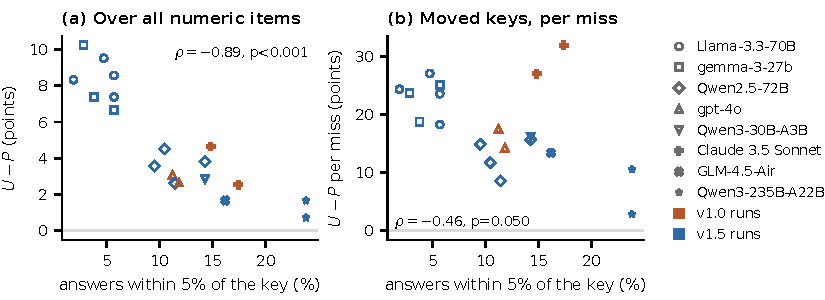
\includegraphics[width=\linewidth]{figures/scaling.pdf}
\caption{\textbf{The cost of a hidden rank falls with agent accuracy, but less per miss.} The nearest-option rule's
$U-P$ for each of the nineteen run sets with the data, against the share of its answers within $5\%$ of the key:
\textbf{(a)} over all numeric items; \textbf{(b)} on the moved keys, per miss (the difference divided by the share of misses
on the moved keys). Markers distinguish the eight models; $\rho$: rank correlation (Spearman's) over the run sets,
with a permutation $p$-value.}
\label{fig:scaling}
\end{figure}

\paragraph{Robustness.} Table~\ref{tab:robust} repeats the main differences on other samples of the runs, other draws of
$U$, other subsets of the items and other graders of the options alone.

\begin{table}[htbp]
\centering\footnotesize
\caption{\textbf{Robustness checks.} Each check, the runs it uses and its result, in points (the rule's $U-P$ on the
moved keys unless stated), with intervals as in Table~\ref{tab:readers2}. A control dataset places the key at random
among options drawn from the dataset's own values, so its options reveal nothing ($\Gamma=0$,
Appendix~\ref{app:theory}).}
\label{tab:robust}
\begin{tabularx}{\linewidth}{@{}>{\raggedright\arraybackslash}p{3.4cm}>{\raggedright\arraybackslash}p{2.6cm}>{\raggedright\arraybackslash}X@{}}
\toprule
check & runs & result\\
\midrule
one run per question, $2{,}000$ draws & published & $15.1$ to $24.6$ in $95\%$ of draws\\
$U$ redrawn with $100$ seeds & v1.5 with and without the data; published & $U$ moves $33$ to $60$ keys to an extreme;
the rule's $U-P$ on them is $+13.4$ to $+24.9$ (v1.5 with the data), $+14.8$ to $+27.9$ (without) and $+16.1$ to
$+29.7$ (published), its interval excluding zero at every seed\\
without the six capsules a concurrent audit examined, three in full and three in a pilot \citep{bixbenchaudit} & all but $23$ of v1.5's $105$ items and $24$ of
v1.0's $159$ & no moved-key difference of the test or of Tables~\ref{tab:readers2} and~\ref{tab:readersfull} changes by
more than $1.8$\\
the keys BixBench-Verified-50's experts re-checked \citep{verified50} & $26$ v1.5 numeric items, $14$ of them moved &
forced-choice excess $+13.5$ $[+6.1,+20.1]$ (seven configurations) and $+15.4$ $[+7.7,+25.3]$ (new seeds); the
rule's $U-P$ $+19.6$ $[+5.0,+31.1]$ and $+19.9$ $[+0.8,+33.3]$\\
without the runs that gave no answer or hit the step, reply-length or time limit & seven configurations, $123$ of $735$ runs
removed & forced-choice excess from $+14.6$ to $+17.3$ $[+14.5,+20.0]$; the rule's $U-P$ from $+16.7$ to $+18.8$
$[+11.7,+25.9]$\\
four more runs of Qwen3-235B-A22B, after the test & $420$ question runs & $+9.5$ $[+0.9,+17.4]$; with the test's two runs
$+7.9$ $[+0.7,+14.7]$; on its $30$ unchanged keys whose rank $U$ leaves as released, $+0.3$\\
the three configurations whose accuracy rises with the data & Qwen2.5-72B (text), GLM-4.5-Air, Qwen3-30B-A3B &
forced-choice excess $+10.8$ $[+5.3,+16.4]$; the rule's $U-P$ $+12.4$ $[+4.8,+21.9]$\\
a learned grader of the options alone: a linear score of features of each option set (ranks, written length,
significant digits), fitted on some capsules and scored on the held-out ones & v1.5's $R$, $P$, $U$ & selects the key on $43.8$, $41.9$
and $30.5\%$; on ten control datasets, whose options cannot reveal the key, on at most $30.5\%$\\
\bottomrule
\end{tabularx}
\end{table}

\FloatBarrier
\subsection{Designs of the options}
\label{app:design}

Every design of \S\ref{sec:design} keeps each numeric item's key and sets its rank: drawn uniformly from all $k$
ranks (\emph{uniform}), from the $k-2$ middle ones, so kept off the extremes (\emph{middle}), or the key's released rank
($k=4$). The generator of $P$ and $U$ (Appendix~\ref{app:options}) draws the $k-1$ distractors, except in the designs
from agents' errors, which take them from the numbers other agents submitted to the same question that are more than
$5\%$ from the key and of its sign; a run is graded through options built without its own model's numbers. We compare
designs on the runs that every design can grade ($4{,}877$ of the $5{,}161$ published runs, and $2{,}070$ of the $2{,}205$ v1.5 runs with the data: the seven
configurations', the new seeds', Qwen3-235B-A22B's six runs per question and gpt-5.1's two). When the options are close together,
keys written with few digits cannot take every rank. So under the middle design the most frequent middle rank holds
more than its uniform share ($35.4$ against $25\%$ of v1.0's keys at $k=6$), and the rank rule gains
more than Observation~\ref{obs:bracket}'s floor
(Table~\ref{tab:design}). Table~\ref{tab:designpairs} sets out what drawing the rank from all $k$ costs.

\begin{table}[htbp]
\centering\scriptsize\setlength{\tabcolsep}{2pt}
\caption{\textbf{Designs of the options.} Each design's distractors, number of options $k$ and key rank; the rank rule's gain over $1/k$ in points, in
theory (Observation~\ref{obs:bracket}'s floor) and on held-out capsules of each release; the share of misses the
nearest-option rule accepts, reading the last number, on the runs every design can grade; and, over the four
answer-only graders, the range of the share of misses they accept (--: not graded) and of correct answers they accept,
over both releases. \emph{Redrawn}: a new draw spaced as $P$ and $U$, each value written with the significant digits of a released
distractor; \emph{a fifth} or \emph{a tenth apart}: at that fraction of the
key; \emph{agents' errors}: from other agents' wrong numbers.}
\label{tab:design}
\resizebox{\linewidth}{!}{\begin{tabular}{lrlrrrrrrrr}
\toprule
& & & \multicolumn{3}{c}{rank rule's gain} & \multicolumn{2}{c}{rule: misses accepted} &
\multicolumn{2}{c}{graders: misses accepted} & graders: correct\\
\cmidrule(lr){4-6}\cmidrule(lr){7-8}\cmidrule(lr){9-10}
distractors & $k$ & key rank & theory & v1.0 & v1.5 & v1.0 & v1.5 & v1.0 & v1.5 & accepted\\
\midrule
$R$, released & $4$ & released & -- & $-2.4$ & $+26.4$ & $18.6$ & $12.5$ & -- & -- & --\\
$P$ & $4$ & released & -- & $-2.8$ & $+26.4$ & $20.4$ & $13.7$ & -- & -- & --\\
$U$ & $4$ & uniform & $0.0$ & $+0.2$ & $-6.9$ & $25.4$ & $23.0$ & -- & -- & --\\
redrawn & $4$ & released & -- & $-2.4$ & $+26.4$ & $21.3$ & $14.6$ & $28.5$--$33.6$ & $20.2$--$24.5$ & $92.9$--$100.0$\\
redrawn & $4$ & uniform & $0.0$ & $+0.2$ & $+0.7$ & $28.1$ & $23.3$ & $34.1$--$38.0$ & $26.9$--$31.0$ & $95.1$--$99.7$\\
redrawn & $4$ & middle & $25.0$ & $+30.1$ & $+20.2$ & $14.8$ & $12.2$ & $20.8$--$27.0$ & $19.0$--$21.3$ & $93.3$--$98.3$\\
redrawn & $6$ & uniform & $0.0$ & $+6.0$ & $-0.5$ & $24.2$ & $22.0$ & -- & -- & --\\
redrawn & $6$ & middle & $8.3$ & $+18.8$ & $+15.1$ & $13.7$ & $12.1$ & -- & -- & --\\
redrawn & $8$ & uniform & $0.0$ & $+1.3$ & $+0.8$ & $22.4$ & $19.0$ & $27.8$--$30.6$ & $21.7$--$24.2$ & $93.7$--$100.0$\\
redrawn & $8$ & middle & $4.2$ & $+9.0$ & $+9.6$ & $14.5$ & $12.2$ & $16.8$--$20.6$ & $14.9$--$15.7$ & $95.3$--$100.0$\\
redrawn & $10$ & uniform & $0.0$ & $-2.5$ & $-4.3$ & $20.8$ & $19.7$ & -- & -- & --\\
redrawn & $10$ & middle & $2.5$ & $+5.2$ & $+11.2$ & $14.4$ & $12.1$ & -- & -- & --\\
a fifth apart & $8$ & uniform & $0.0$ & $+0.1$ & $+7.7$ & $13.3$ & $14.6$ & -- & -- & --\\
a fifth apart & $8$ & middle & $4.2$ & $+13.4$ & $+10.6$ & $5.8$ & $6.1$ & $11.0$--$12.8$ & $10.5$--$13.0$ & $92.0$--$100.0$\\
a tenth apart & $8$ & middle & $4.2$ & $+7.9$ & $+14.7$ & $3.6$ & $3.7$ & -- & -- & --\\
agents' errors & $4$ & released & -- & $-0.3$ & $+28.5$ & $19.1$ & $15.4$ & $24.5$--$27.5$ & $19.0$--$19.5$ & $92.9$--$99.7$\\
agents' errors & $4$ & uniform & $0.0$ & $-7.7$ & $+1.7$ & $26.2$ & $25.3$ & $29.8$--$30.6$ & $26.0$--$28.6$ & $91.6$--$98.4$\\
agents' errors & $4$ & middle & $25.0$ & $+31.8$ & $+22.0$ & $13.2$ & $14.4$ & -- & -- & --\\
\bottomrule
\end{tabular}}
\end{table}

\begin{table}[htbp]
\centering\scriptsize\setlength{\tabcolsep}{2pt}
\caption{\textbf{What drawing the rank from all $k$ costs.} How many more answers, in points, the nearest-option rule accepts when the key's rank is drawn
from all $k$ ranks than when it is released or kept off the extremes: on the keys this moves from bracketed to extreme
(their number on v1.0 and v1.5), with intervals as in Appendix~\ref{app:stats}, and over all items; and the range of
the same difference on those keys over the four answer-only graders (--: not graded). Here the rule reads the last number, on the runs every design can grade, so its $U-P$
differs from Table~\ref{tab:cost}'s.}
\label{tab:designpairs}
\resizebox{\linewidth}{!}{\begin{tabular}{lrrrrrrr}
\toprule
& moved & \multicolumn{2}{c}{rule: moved keys} & \multicolumn{2}{c}{rule: all items} &
\multicolumn{2}{c}{graders: moved keys}\\
\cmidrule(lr){3-4}\cmidrule(lr){5-6}\cmidrule(lr){7-8}
design & keys & v1.0 & v1.5 & v1.0 & v1.5 & v1.0 & v1.5\\
\midrule
$U-P$ & $40$, $37$ & $+22.2$ {\scriptsize$[+11.5,+35.1]$} & $+18.7$ {\scriptsize$[+11.1,+25.4]$} & $+4.7$ & $+6.1$ & -- & --\\
$k=4$, uniform $-$ released rank & $56$, $44$ & $+24.9$ {\scriptsize$[+18.3,+32.4]$} & $+18.1$ {\scriptsize$[+12.2,+25.0]$} & $+5.4$ & $+6.1$ & $+21.0$--$+30.5$ & $+16.9$--$+19.3$\\
agents' errors, uniform $-$ released rank & $47$, $34$ & $+24.1$ {\scriptsize$[+16.3,+33.8]$} & $+18.8$ {\scriptsize$[+11.3,+28.1]$} & $+5.9$ & $+7.7$ & $+17.7$--$+25.1$ & $+19.6$--$+27.2$\\
$k=4$, uniform $-$ middle & $88$, $53$ & $+21.2$ {\scriptsize$[+16.1,+26.3]$} & $+16.2$ {\scriptsize$[+10.9,+22.5]$} & $+11.1$ & $+8.4$ & $+16.3$--$+26.2$ & $+14.1$--$+21.5$\\
$k=6$, uniform $-$ middle & $60$, $36$ & $+21.9$ {\scriptsize$[+16.3,+27.7]$} & $+23.0$ {\scriptsize$[+17.1,+29.0]$} & $+9.0$ & $+7.1$ & -- & --\\
$k=8$, uniform $-$ middle & $41$, $23$ & $+23.8$ {\scriptsize$[+17.9,+30.0]$} & $+21.7$ {\scriptsize$[+11.3,+30.4]$} & $+6.1$ & $+4.5$ & $+28.5$--$+30.2$ & $+24.0$--$+27.0$\\
$k=10$, uniform $-$ middle & $35$, $23$ & $+25.2$ {\scriptsize$[+15.7,+36.3]$} & $+26.3$ {\scriptsize$[+14.9,+39.6]$} & $+5.6$ & $+5.8$ & -- & --\\
$k=8$, a fifth apart, uniform $-$ middle & $37$, $29$ & $+23.4$ {\scriptsize$[+15.6,+32.1]$} & $+19.9$ {\scriptsize$[+12.8,+27.4]$} & $+5.7$ & $+5.8$ & -- & --\\
\bottomrule
\end{tabular}}
\end{table}

\end{document}
